\documentclass[a4paper,12pt]{article}
\usepackage{amsmath,graphicx}
\usepackage[font={scriptsize}]{caption}
\usepackage{cite}

\graphicspath{{images/}}
\begin{document}
\bibliographystyle{naturemag}
\begin{titlepage}
\date {Academic Year 2013-2014 Semester 2}
\newcommand{\HRule}{\rule{\linewidth}{0.5mm}} % Defines a new command for the horizontal lines, change thickness here
\center % Center everything on the page
\textsc{\LARGE National University of Singapore}\\[1.5cm]
\textsc{\Large Faculty of Science/University Scholars Program}\\[0.5cm]
\textsc{\large UIS3921 Independent Study Module}\\[0.5cm]
\HRule \\[0.4cm]
{ \huge \bfseries Cell line selection using genomic profiles}\\[0.4cm]
\HRule \\[1.5cm]
\begin{minipage}{0.4\textwidth}
\begin{flushleft} \large
\emph{Author:}\\
\textsc{Ng} Wee Kiat Jeremy
\end{flushleft}
\end{minipage}
~
\begin{minipage}{0.4\textwidth}
\begin{flushright} \large
\emph{Supervisor:} \\
Professor Greg-Tucker \textsc{Kellogg}
\end{flushright}
\end{minipage}\\[4cm]


{\large Academic Year 2013-2014 Semester 2}\\[3cm] % Date, change the \today to a set date if you want to be precise


%\includegraphics{Logo}\\[1cm] % Include a department/university logo - this will require the graphicx package


\vfill % Fill the rest of the page with whitespace

\end{titlepage}
\newpage
\tableofcontents
\newpage
\listoffigures
\listoftables
\newpage
\addcontentsline{toc}{section}{Abstract}
\begin{abstract}
Cancer cell lines serve as invaluable $\textit{in vitro}$ models for
researchers. Today, there is a large number of available cell lines
for the study of different cancer subtypes. Yet, no guidelines exist
to aid the selection of cell lines in experimental studies. Using
publicly available data from The Cancer Genome Atlas (TCGA) and Cancer
Cell Line Encyclopedia (CCLE), Domcke et al proposed a scoring scheme
using copy number variation data and somatic mutation data to select a
most suitable cell line for the study of ovarian cancer. In this
present study, we refine Domcke et al's scoring scheme further by
introducing a new scoring scheme that also includes information from
gene expression profiles as well as a weighted scoring component for
somatic mutations. We then apply our method to identify a suitable
cell line model for the study of $\textit{TGF}$-$\beta$ sensitive
breast cancer.
\end{abstract}

\newpage
\section{Introduction}
Breast cancer is one of the most common cancers worldwide, with an
estimated 1,300,000 new cases and 450,000 deaths reported
annually. Clinically,  breast cancer is classified into three distinct
subtypes based on their eostrogen receptor status. Namely, breast
cancer is defined along the expression of the $\textit{HER}$,
$\textit{ER}$ and $\textit{PR}$ receptors. This classification
has been helpful in devising therapeutic regimes, as different
receptor statuses lead to differing response to chemotherapy regimes\cite{Rouzier2005}. However, there are other pathways that are
relevant in determining drug response. One such pathway is that of the
$\textit{TGF}$-$\beta$ pathway, which is particularly important in
determining patient response to antihormonal treatment in $\textit{ER}$-positive breast cancer \cite{knabbe1987}.

$\textit{TGF}$-$\beta$ is a growth factor that has a wide range of
effects, including the suppression of tumorigenesis \cite{yang2010}. The canonical pathway of $\textit{TGF}$-$\beta$ involves the binding of
$\textit{TGF}$-$\beta$ to $\textit{SMAD}$ proteins, in which the
activated $\textit{SMAD}$ protein then serves as a transcription
factor (Figure \ref{SMAD}).
\begin{figure}[htbp!]
\centering
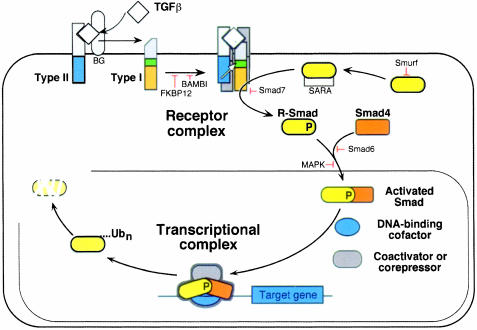
\includegraphics[width=7cm]{smad.jpg}
\caption[Diagram showing the $\textit{TGF}$-$\beta$/$\textit{SMAD}$
pathway]
{Diagram showing the $\textit{TGF}$-$\beta$/$\textit{SMAD}$
  pathway. Upon activation and dimerization of the
  $\textit{TGF}$-$\beta$ receptor, $\textit{SMAD}$-4 is then
  activated, which is then transported into the nucleus to serve as a
  transcription factor. Taken from Massague and Wotton, 2000.}
\label{SMAD}
\end{figure}
Despite the fact that  $\textit{TGF}$-$\beta$ normally
functions as a tumor suppressor, it is also recognized that in the
later stages of cancer,  $\textit{TGF}$-$\beta$ instead becomes a
promoter of tumor progression, stimulating angiogenesis, inducing
extracellular matrix degradation and inhibiting antitumor immune
response \cite{McEarchern2001,Bierie2006}. Likewise,
$\textit{TGF}$-$\beta$ is known to activate other signaling pathways
to module the $\textit{TGF}$$\beta$-$\textit{SMAD}$ response \cite{Zhang2009}. Therefore, the $\textit{TGF}$-$\beta$ pathway is an
attractive target of study as one can imagine a therapy which aims to
reverse the oncogenic effect of $\textit{TGF}$-$\beta$, and hence
restoring $\textit{TGF}$-$\beta$ as a tumor suppressor.

Cell lines are popular $\textit{in vitro}$ models that have been
instrumental in furthering our understanding of cancer biology. Apart
from helping us gain insights into the mechanisms of disease
progression, cancer cell lines are also used extensively to screen for
potential anti-cancer drugs \cite{Yamori2003}. Earlier studies have
highlighted the many uncertainties that plague cell line selection,
such as the risk of cross contamination \cite{Gillet2013} or
cell lines of unknown origin that are mistaken for a wrong cancer type
\cite{Domcke2013}.  There is thus great interest in ensuring that
the cell line models that are selected are as identical to the actual
cancer type in question.  One potential criteria for the selection of
the most appropriate cell line is the use of genomic data as the
basis by which cell lines are selected.

Although the use of genomic data to guide cell line selection
is not entirely novel, earlier efforts were concentrated on using only one type of
genomic data. For instance, Sandberg and Ernberg (2005) devised the
Tissue Similarity Index (TSI) as a measure of how similar a cell line is to
a tumor sample, in which they used Singular Value Decomposition to
identify similar gene expression profiles
\cite{sandberg2005}.  Attempts to integrate
multiple data types have been hampered by the lack of comprehensive
characterization of tumors and cell line models. Indeed, the first
attempt to integrate genomic data from multiple platforms was only
made in wake of the extensive characterization of tumor samples by
The Cancer Genome Atlas (TCGA), as well as the availability of genomic
information of cell lines in the Cancer Cell Line Encyclopedia (CCLE). In their work, Domcke et al proposed a scoring scheme to guide cell line selection. In
particular, they proposed cell line suitability to be defined by the
formula\begin{equation} S = A + B - 2 \times C - \frac{D}{7}\end{equation},where A is
the correlation with the mean CNA of HGSOC tumours, B is 1 for cell
lines harbouring a TP53 mutation and 0 otherwise, C is 1 for
hypermutated cell lines and 0 otherwise, and D is the number of genes
mutated among the seven ‘non-HGSOC’ genes recurrently altered only in
the other ovarian cancer subtypes.

However, one noticeable inadequacy of the method proposed by Domcke et
al is that gene expression patterns were not considered. This is
particularly significant because it has been shown in other studies
that gene expression patterns can be used to define cancer subtypes as
well as the therapeutic response of patients \cite{Veer2002,Finetti2004,Finetti2005}. Further scrutiny of the scoring scheme proposed by Domcke et al
also yields another inadequacy; that is, the penalty for the
differences in mutation profile between the cell line and the tumor
samples are not weighted. As a consequence, the scheme applies an
equal penalty to a cell line that has the absence of a near universal mutation and the absence of a rarer mutation (in the
$\frac{D}{7}$ scoring component). In this present study, we attempt to
refine the scoring scheme proposed by Domcke et al, addressing the two
inadequacies that we have identified in their earlier scoring
scheme. We then apply our method to guide our selection of a suitable
cell line for the study of $\textit{TGF}$-$\beta$ sensitive breast cancer.

\section{Methods and Materials}
\subsection{Data acquisition}
All data obtained are publicly available from the TCGA portal and the
CCLE portal. For tumor data, we select only samples which have gene
expression data in the form of RNASeq, CNV data and data on somatic
mutation. There is no requirement for the samples to be normal-tumor
matched. We use TCGA Level 3 data, which is extensively processed and
summarized - with the exception of somatic mutations, in which data is
provided up to only Level 2. In all, data for 936 samples from TCGA were
downloaded. Similarly, processed CCLE data for gene expression, CNV
arrays and somatic mutation were downloaded. Data for a total of 1037 cell lines
were downloaded from CCLE.

\subsection{Softwares}
All work was done using the freely available R software (version
3.02). Additional packages were downloaded from either the
Comprehensive R Archive Network (CRAN) or the $\textit{BioConductor}$
repository. The codes used for the analysis in this paper are made
publicly available on $\textit{Github}$.

\subsection{Validation  of batch effects}
In particular, because TCGA data is processed across numerous batches,
it is thus important to ensure that there are no distinct batch
effects. We perform principal component analysis using the R package
$\textit{FactoMineR}$(Francois et al, 2013), and then cluster the
samples according to the first and second principle component (PC1 and PC2,
respectively). Visualization is done using a contour map that was
generated using a $\textit{Python}$ module $\textit{matplotlib}$.

\subsection{Clustering}
Clustering was performed using the Ward agglomerative algorithm as
implemented in R, using a Euclidean distance matrix.
Prior to cluster analysis, feature selection was first performed to
reduce the number of gene features that were used for
clustering. Briefly, we first used the $\textit{TGF}$-$\beta$ gene set
available from Broad Institute to select for genes that are known to
be regulated by $\textit{TGF}$-$\beta$. This reduced the total number
of gene of interest from about 20,000 genes to 372 genes. Thereafter,
all the RNASeq data was log$_2$-transformed and
$\textit{z}$-normalized so that all the samples have a mean of 0 and a
standard deviation of 1. Because there are genes in which there are no
reads, we perform the log-2 transformation as follows \begin{equation} N =
log_2(M+1)\end{equation} where N is a matrix of log-transformed reads, and M is
the original matrix of reads from RSEM-normalization. Thereafter, we
estimate the variability R of each gene \textit{g} in sample
\textit{s} as follows \begin{equation} R= \frac{\textit{g}_s}{\mu \textit{g}} \end{equation}Finally, the standard deviation of each gene across all the samples
were calculated, and the top 20 most variable genes with the largest
standard deviations were selected as features for clustering.

\subsection{Analysis of gene expression}
Following clustering, we then identified a sub-group of samples that
are most representative of $\textit{TGF}$-$\beta$ sensitive tumor
samples. The gene expression profile of the $\textit{TGF}$-$\beta$ was
then estimated by taking the median of all the 372 genes known to be
regulated by $\textit{TGF}$-$\beta$. Similarity between the tumor
model and cell line was measured using the Spearman $\rho$.

\subsection{Analysis of copy number aberrations}
The package $\textit{BioConductor}$ package $\textit{CNtools}$ (Zhang,
2013) was used to summarize CNV data from TCGA by genes. Thereafter, we
constructed a representative profile by taking the medians of all the
CNV counts for each gene across all the samples of interest. Following
the lead of Domcke et al, similarity between the tumor model and the
cell lines  was measured using the Pearson $\textit{r}$.

\subsection{Analysis of mutations}
The curated somatic mutation provided by TCGA is used for downstream
analysis. In order to estimate the probability of the sample being
from a $\textit{TGF}$-$\beta$ sensitive origin based on the somatic
mutation, we employ the Bayes theorem. Formally, let P($\textit{X}$)
denote the probability of the sample being $\textit{TGF}$-$\beta$
sensitive, and P($\textit{Y}$) be the probability of a sample having a
collection of mutations, we can denote P($\textit{X}$$\mid$$\textit{Y}$) as \begin{equation}
P(\textit{X}\mid \textit{Y}) = P(\textit{Y}\mid\textit{X})\times
\dfrac{P(\textit{X})}{P(\textit{Y})} \end{equation}We use the TCGA data to derive the required prior probabilities. In
particular,
\begin{equation}
P(\textit{X})=\dfrac{n(\textit{TGF}\beta \;\; sensitive\;\; samples)}{n(samples)}
\end{equation}In order to define P($\textit{Y}$), let the vector $\phi$ be
the vector of mutation frequency in genes $\textit{1}$ to $\textit{k}$ ; that
is, \[\phi=(\textit{F}_1, ... , \textit{F}_k) \] where
$\textit{F}$$_i$ is the mutation frequency of gene $\textit{i}$
observed in the TCGA dataset. We define $\textit{F}$$_i$ as \begin{equation}
\textit{F}_i = \dfrac{n(mutations \;\; at\;\; loci \;\; \textit{i})}{n(samples)}
\end{equation}
Assuming that mutations occur randomly, we can derive P($\textit{Y}$)
for a given cell line as \begin{equation} P(\textit{Y}) = \textit{F}_1
\times \textit{F}_2 \times \textit{F}_3 \times
\textit{F}_4 \times ... \times \textit{F}_k\end{equation}
The last probability term, P($\textit{Y}$$\mid$$\textit{X}$)
represents the probability of a particular mutation profile given that
the sample is known to be $\textit{TGF}$-$\beta$ sensitive. This is
also derived from TCGA is defined similar to (7). However,
unlike (7) where the mutation frequencies are calculated from
all the samples, the mutation frequencies are now calculated only from
the $\textit{TGF}$-$\beta$ responsive samples. For simplicity, we refer
to the conditional probability P($\textit{X}$$\mid$$\textit{Y}$) as $\textit{p}$.

\subsection{Scoring and cell line selection}
A suitable scoring function is one that will capture the similarities
(and differences) in genomic profile between the tumor model and the
cell lines. We define the score of a cell line, $\textit{S}$$_c$ as \begin{equation}
\textit{S}_c= \rho + \textit{r} + \textit{p} +2 \end{equation}, where $\rho$
represents the correlation of gene expression, $\textit{r}$ represents
the correlation of CNV and $\textit{p}$ represents the probability of
a mutation given mutation profile. $\textit{S}$$_c$ can take on the
range of value from 0 to 5, where a higher $\textit{S}$$_c$ suggests a
better cell line model for the system of interest.

\begin{figure}[t!]
\centering
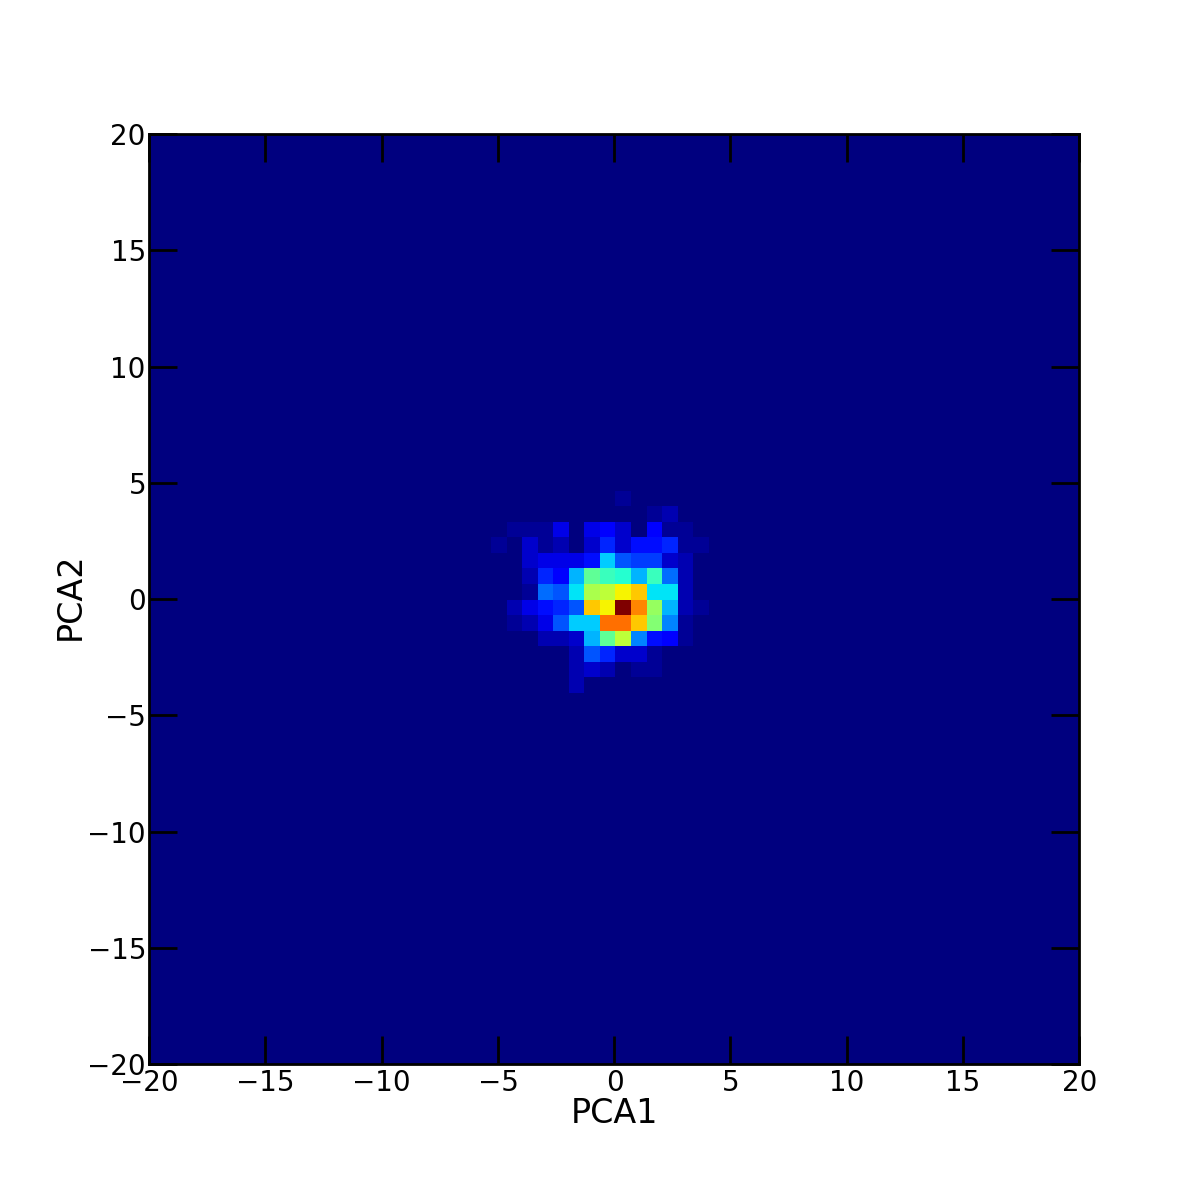
\includegraphics[width=7cm]{PCAplot.png}
\caption[PCA plot of PC1 and PC2 on TCGA RNASeq data]{PCA contour plot
showing the clustering of the RNASeq data from 936 TCGA samples of
multiple batches. There is only one dominant cluster (red), hence
indicating the absence of batch effects. Any differences can thus be
attributed to biological differences.}
\label{pca}
\end{figure}

\section{Results and Discussion}
\subsection{TCGA data does not demonstrate batch effects}
Batch effects serve as a potential confounder in downstream analysis,
and must thus be detected and corrected prior to further downstream
analysis. Batch effects arise due to technical differences - thus
providing a source of variation that is non-biological in origin. This
is an especially valid concern for TCGA data, which is processed in
multiple batches. To test for batch effect, we perform principal
component analysis, and then cluster along the first and second
principal components (PC1 and PC2), and represent them in a contour
plot (Figure \ref{pca}).
From Figure \ref{pca}, we observe only 1 centroid, suggesting that all
the 936 samples cluster well together and hence indicating an absence
of batch effect. Therefore, no correction will be performed on the raw
TCGA data prior to downstream analysis.

\subsection{Clustering of $\textit{TGF}$-$\beta$ sensitive samples occurs along the
  expression of $\textit{SCGB1D2}$}
Following feature selection and clustering, we visualize the 20 genes
using a heatmap (Figure \ref{heatmap}).The samples can be clustered
into 2 major clusters, indicated by the top color bars in Figure
\ref{heatmap}.

\begin{figure}[t]
\centering
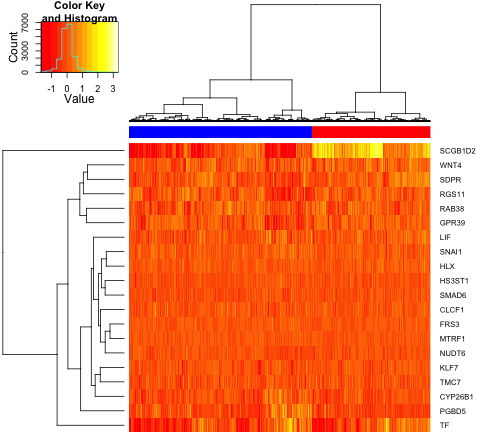
\includegraphics[width=7cm]{heatmap.png}
\caption[Heatmap showing clustering of the top 20 most variable genes]
{Heatmap showing the clustering and the expression of the 20 most
  variable genes in $\textit{TGF}$-$\beta$ response. The top dendrogram
shows the sample clustering, while the side dendrogram shows the
gene clustering.}
\label{heatmap}
\end{figure}
Interestingly, when we turn to the gene clustering, we
notice that the main feature that appears to distiguish between both
groups is the expression of the gene
$\textit{SCGB1D2}$. Significantly, the expression of
$\textit{SCGB1D2}$ is lower in the cluster color-coded blue. This is
shown in Figure \ref{scgb1d2}.
\begin{figure}[h]
\centering
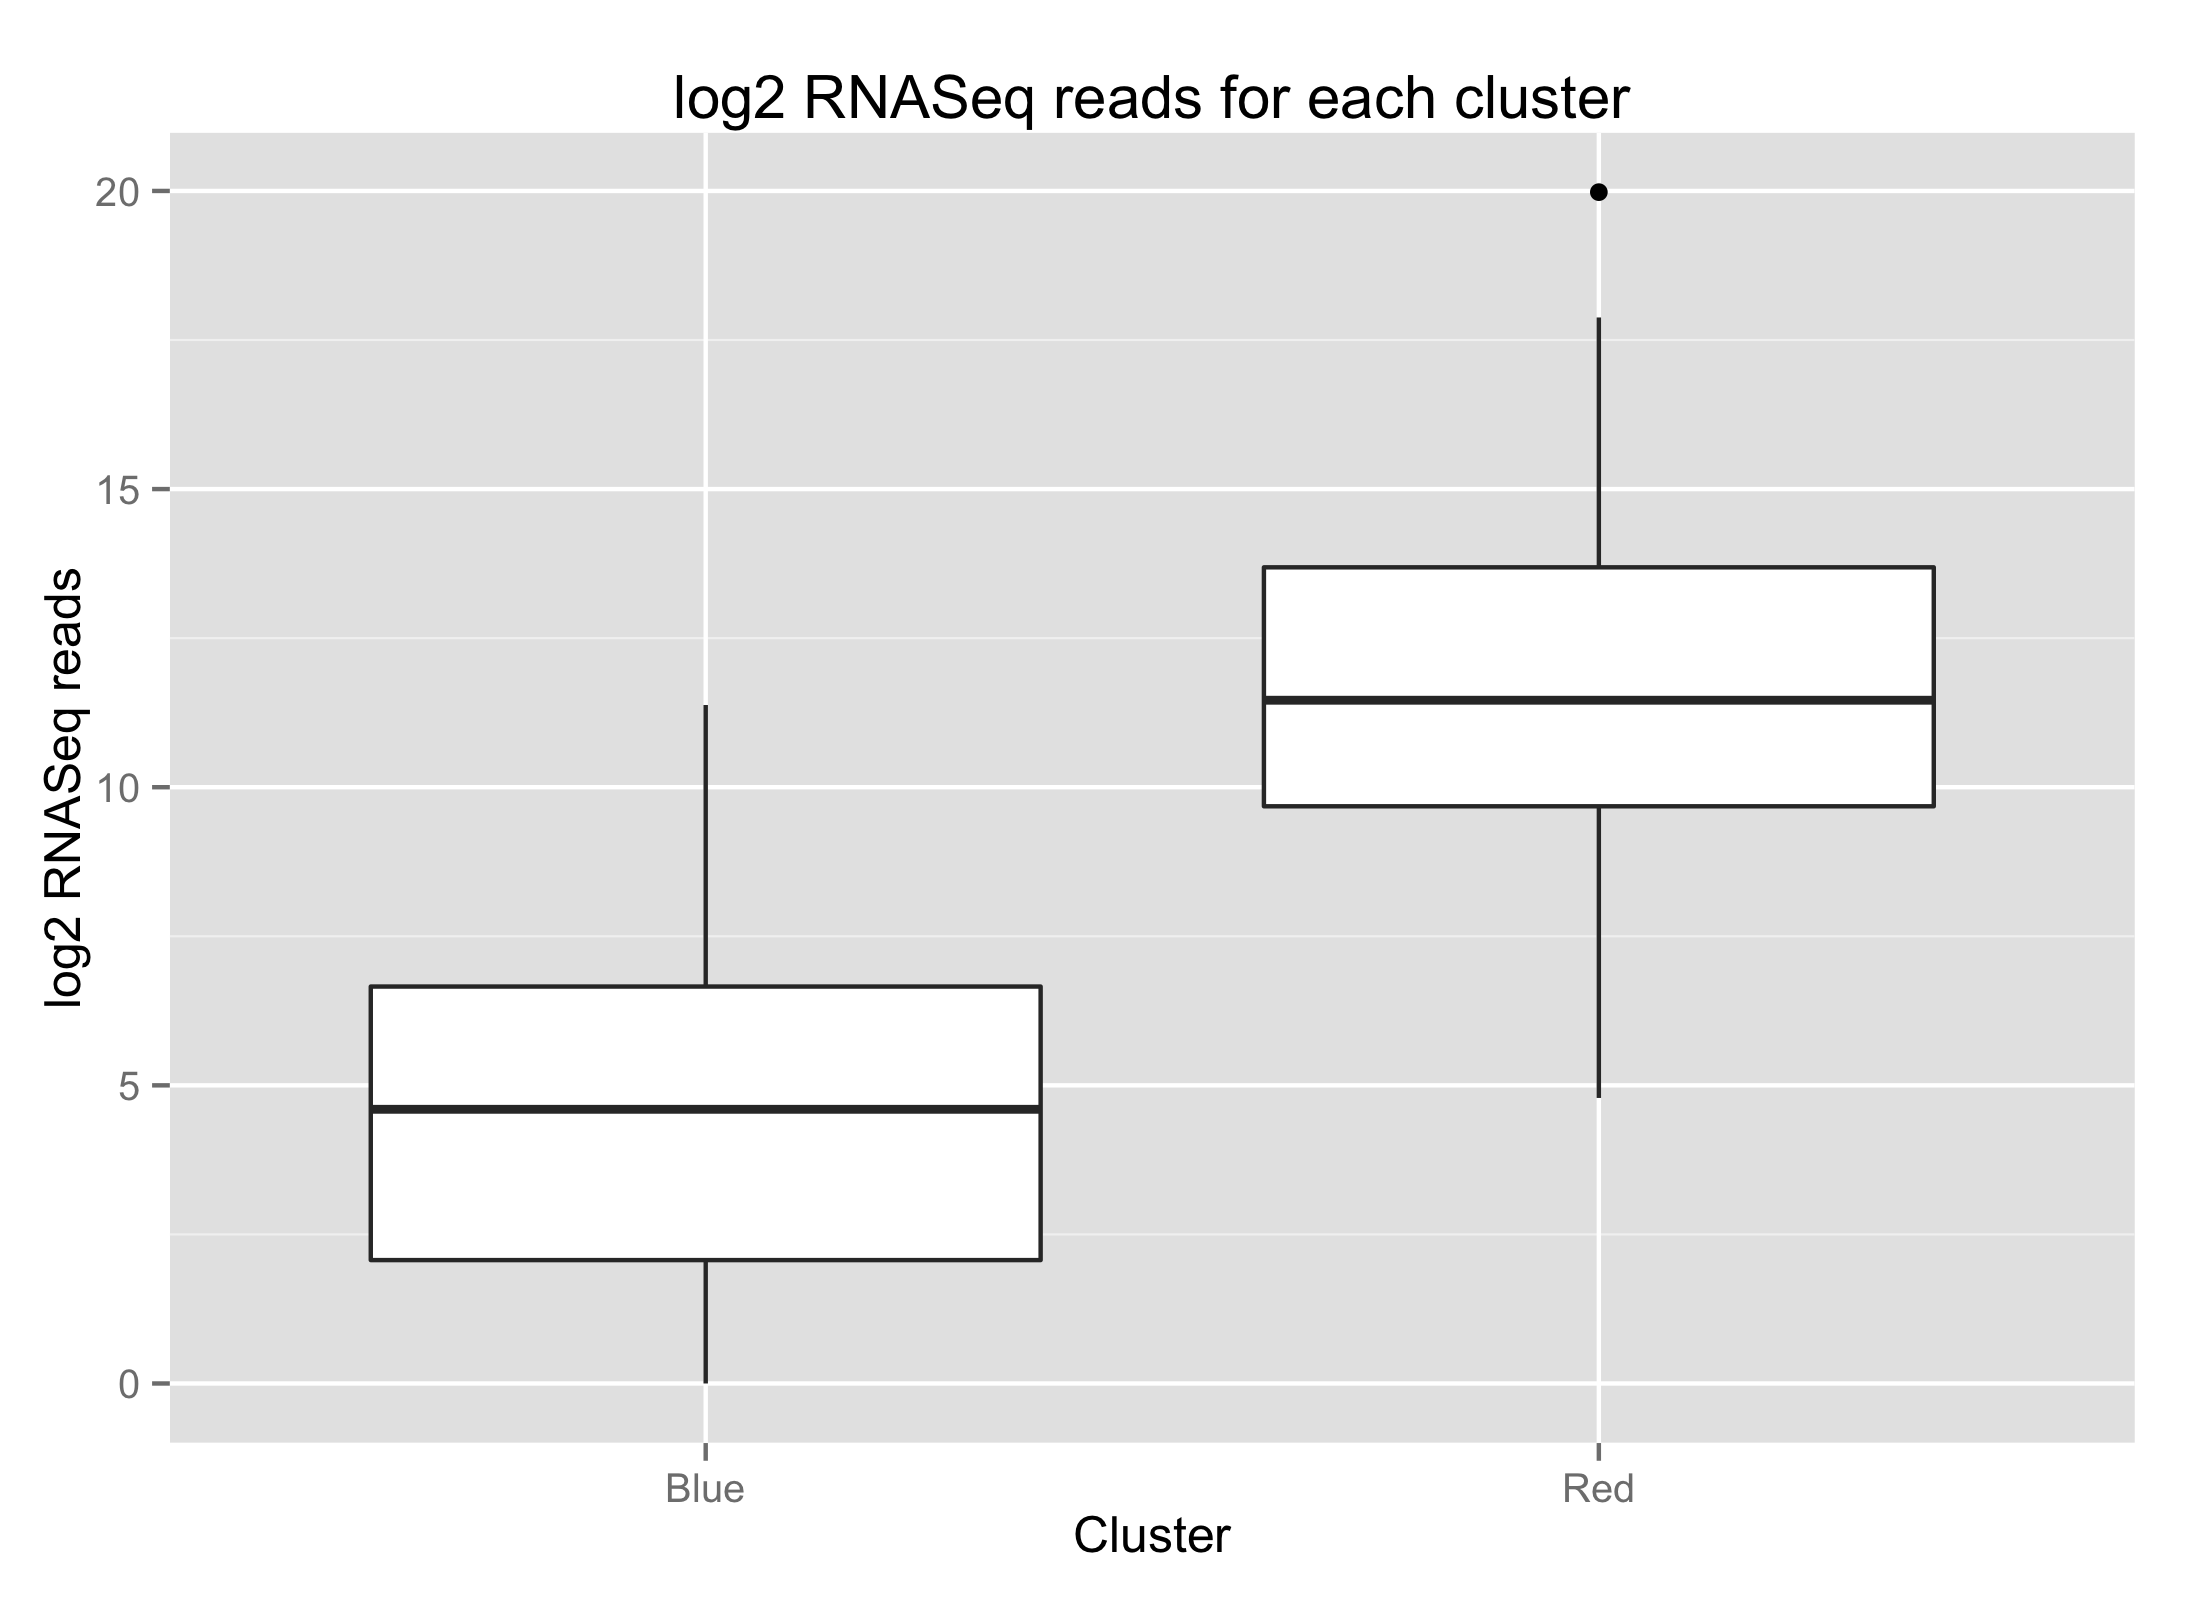
\includegraphics[width=7cm]{rnaseqscgb1d2.png}
\caption[Boxplots of $\textit{SCGB1D2}$ between dominant clusters in
TCGA data]{Boxplot showing the gene expression of the gene
  $\textit{SCGB1D2}$ in the two dominant clusters identified in Figure
\ref{heatmap}.The blue cluster (left) has a significantly lower (p $<$
0.001) expression of  $\textit{SCGB1D2}$ as compared to the red
cluster (right).}
\label{scgb1d2}
\end{figure}
$\textit{SCGB1D2}$ has been shown to be downregulated in 59\% of
breast cancer cases \cite{Zafrakas2006}. This is observed also in
the CCLE dataset, where 59 cell lines annotated as being of breast origin showed a
significantly lower expression of the $\textit{SCGB1D2}$ gene (Figure
\ref{scgb1d2ref}). However, as noted in Figure \ref{scgb1d2ref}, the
expression of $\textit{SCGB1D2}$ is highly variable, with some breast
cell lines having extremely high levels of $\textit{SCGB1D2}$
expression. This observation is consistent with the clustering shown
in Figure \ref{heatmap}, which shows high variability in expression
that allows us to distinguish between subtypes of breast cancers.
\begin{figure}[htbp!]
\centering
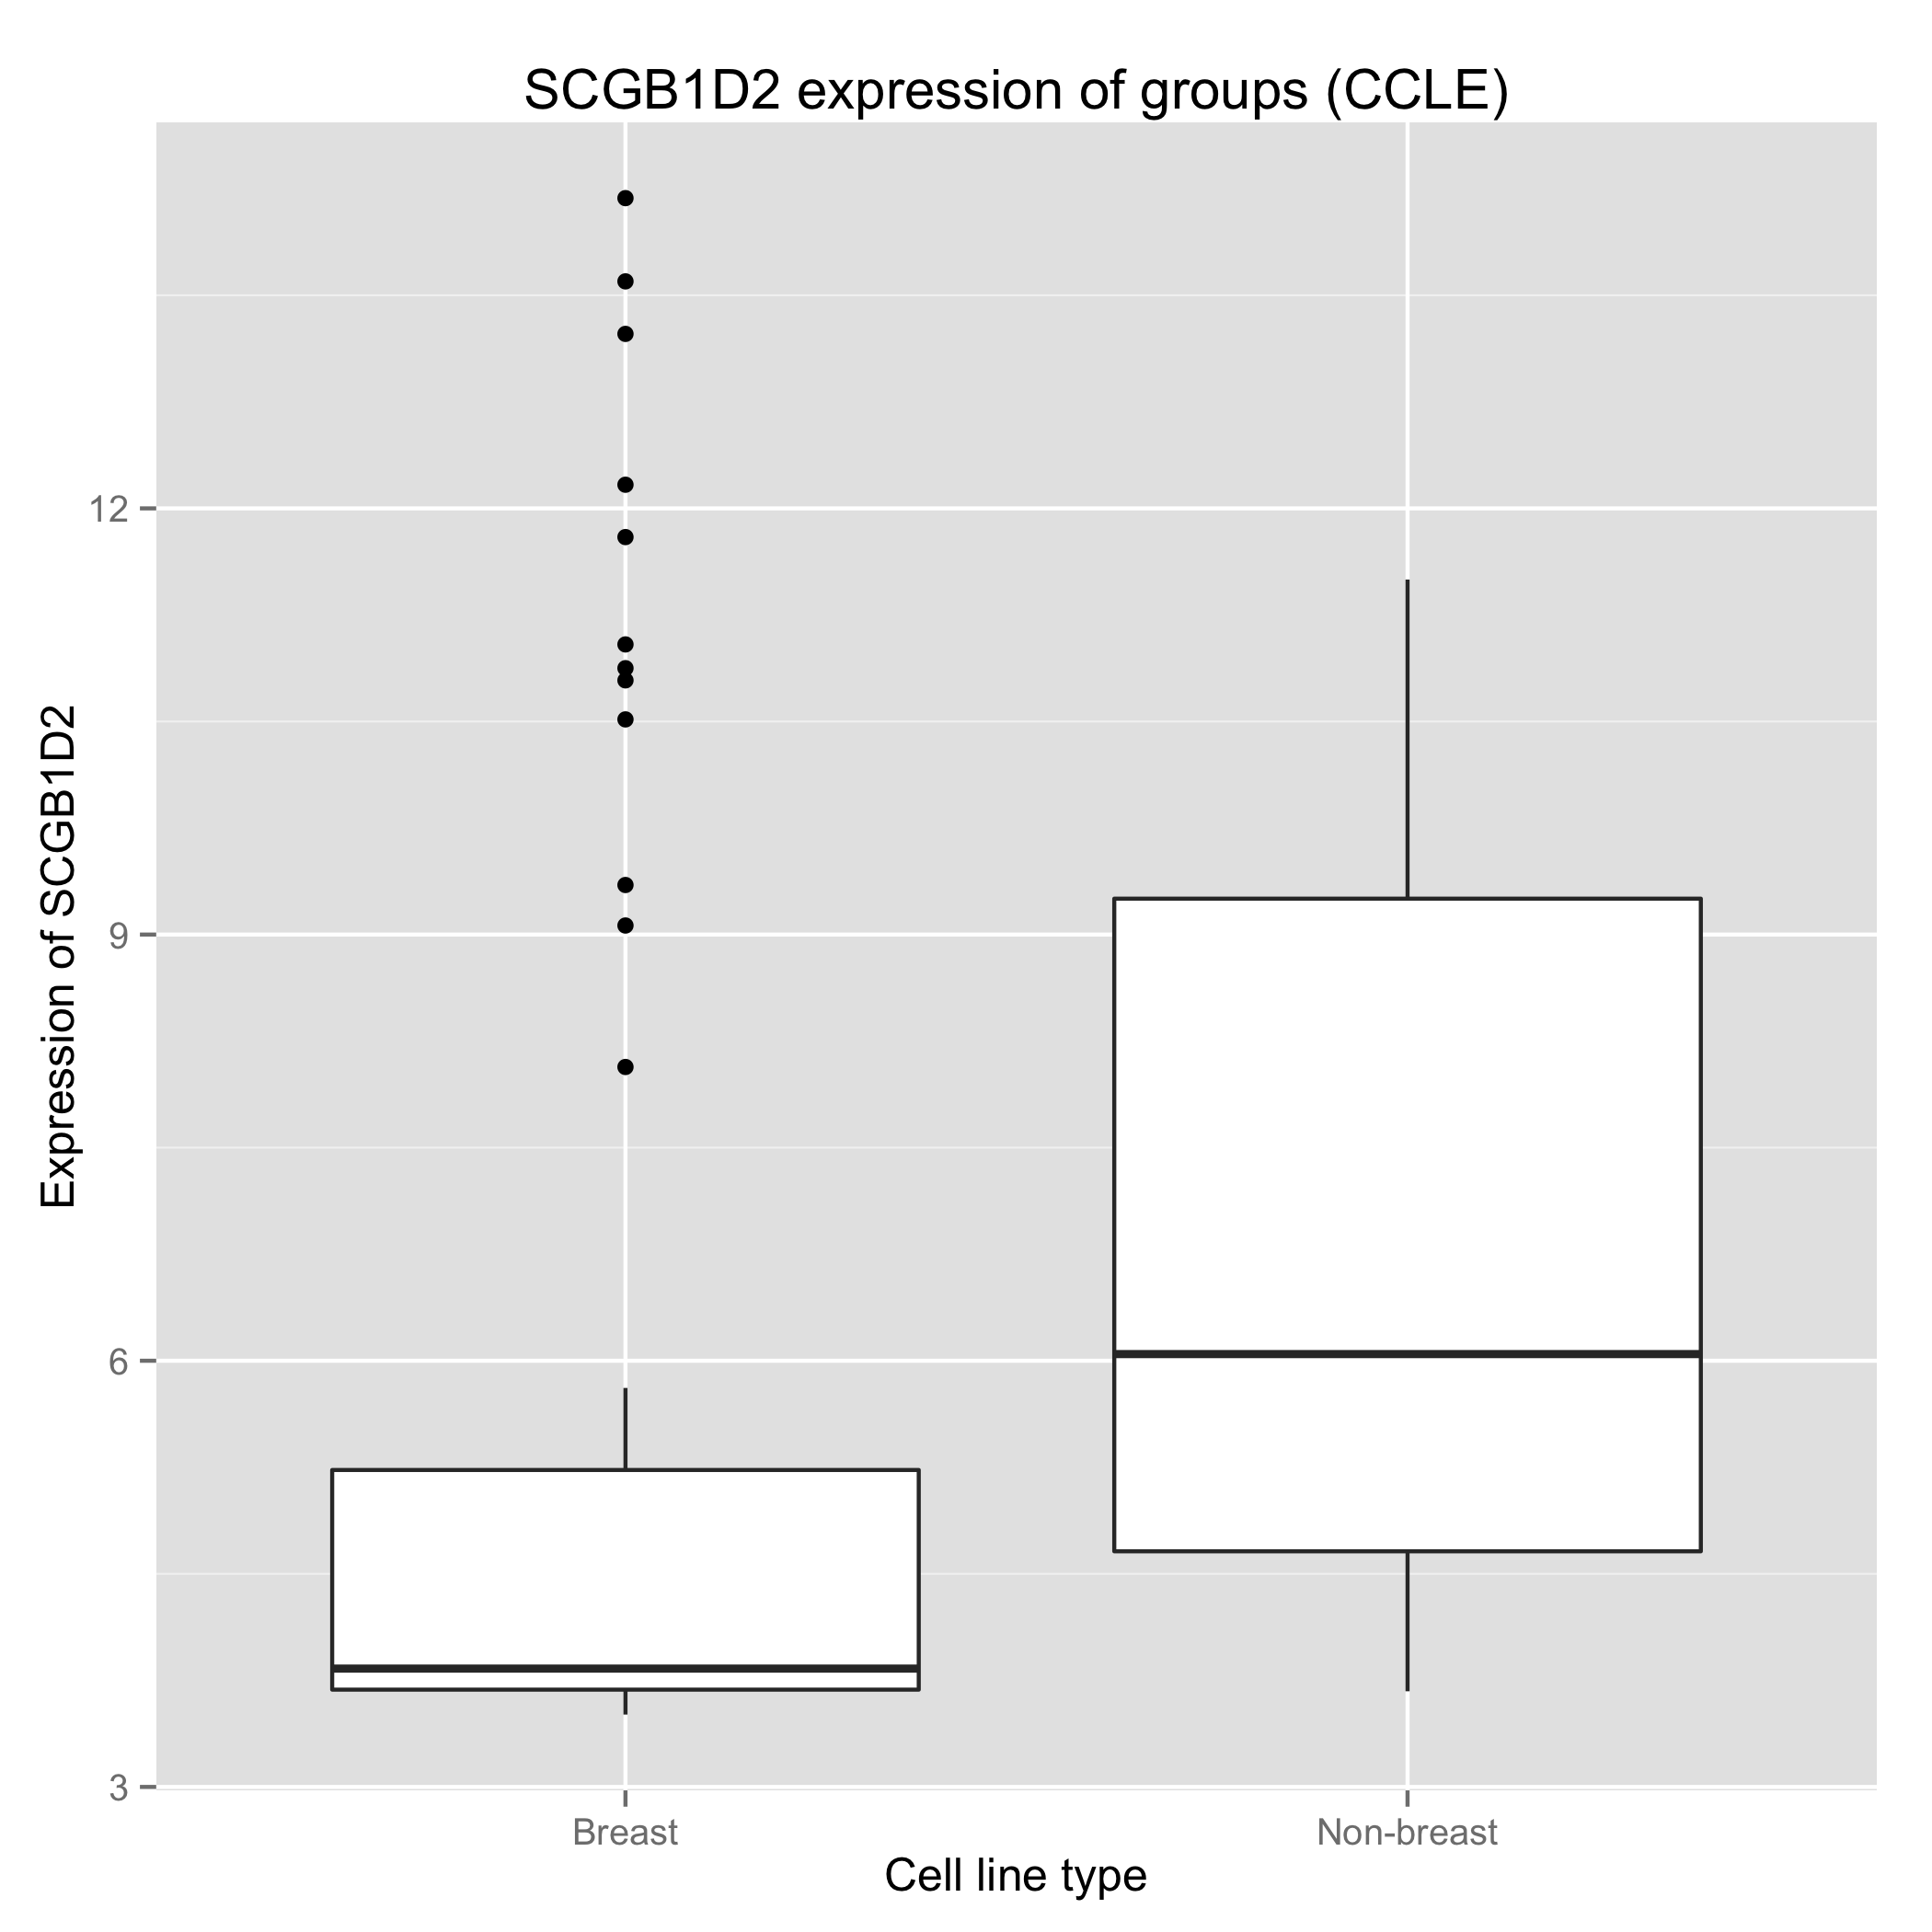
\includegraphics[width=7cm]{scgb1d2expression.png}
\caption[Boxplots of $\textit{SCGB1D2}$ between cell lines of breast
and non-breast origins]{Boxplot showing the expression of
  $\textit{SCGB1D2}$ gene in cell lines of breast and non-breast
  origin. Consistent with earlier studies, the $\textit{SCGB1D2}$ gene
is expressed at lower levels as compared to cell lines of non-breast origin.}
\label{scgb1d2ref}
\end{figure}
In order for us to determine which cluster best represents the
$\textit{TGF}$-$\beta$ sensitive samples, we turn to examine the
nature of interaction between $\textit{TGF}$-$\beta$ and
$\textit{SCGB1D2}$. From the gene sets provided by Broad Institute, we
note that $\textit{SCGB1D2}$ is downregulated by
$\textit{TGF}$-$\beta$, and therefore, we selected the cluster with
the lowest $\textit{SCGB1D2}$ expression to represent the  $\textit{TGF}$-$\beta$
sensitive samples. From the clustering presented in Figure
\ref{heatmap}, we identify a total of 568 samples as being
$\textit{TGF}$-$\beta$ sensitive.

\subsection{Gene expression can be compared using Spearman $\rho$}
We first consider the different platforms used by TCGA and CCLE; in
particular, TCGA uses RNASeq to quantify gene expression while CCLE
uses a single channel Affymetrix U133-2+ chip. Earlier studies by Guo
et al \cite{Guo2013} have demonstrated that data from RNASeq and single
channeled Affymetrix data is highly concordant, with reported Spearman
correlation coefficient of up to 0.9. Likewise, similar to Guo et al,
we use the Spearman $\rho$ as a measure to determine the similarity
between the tumor model and a cell line. Figure \ref{rho} shows
that the observed $\rho$ of cell lines of breast origin (mean=0.75) is higher than
those of non-breast origin (mean=0.71) (p $<$0.001).
\begin{figure}[b!]
\centering
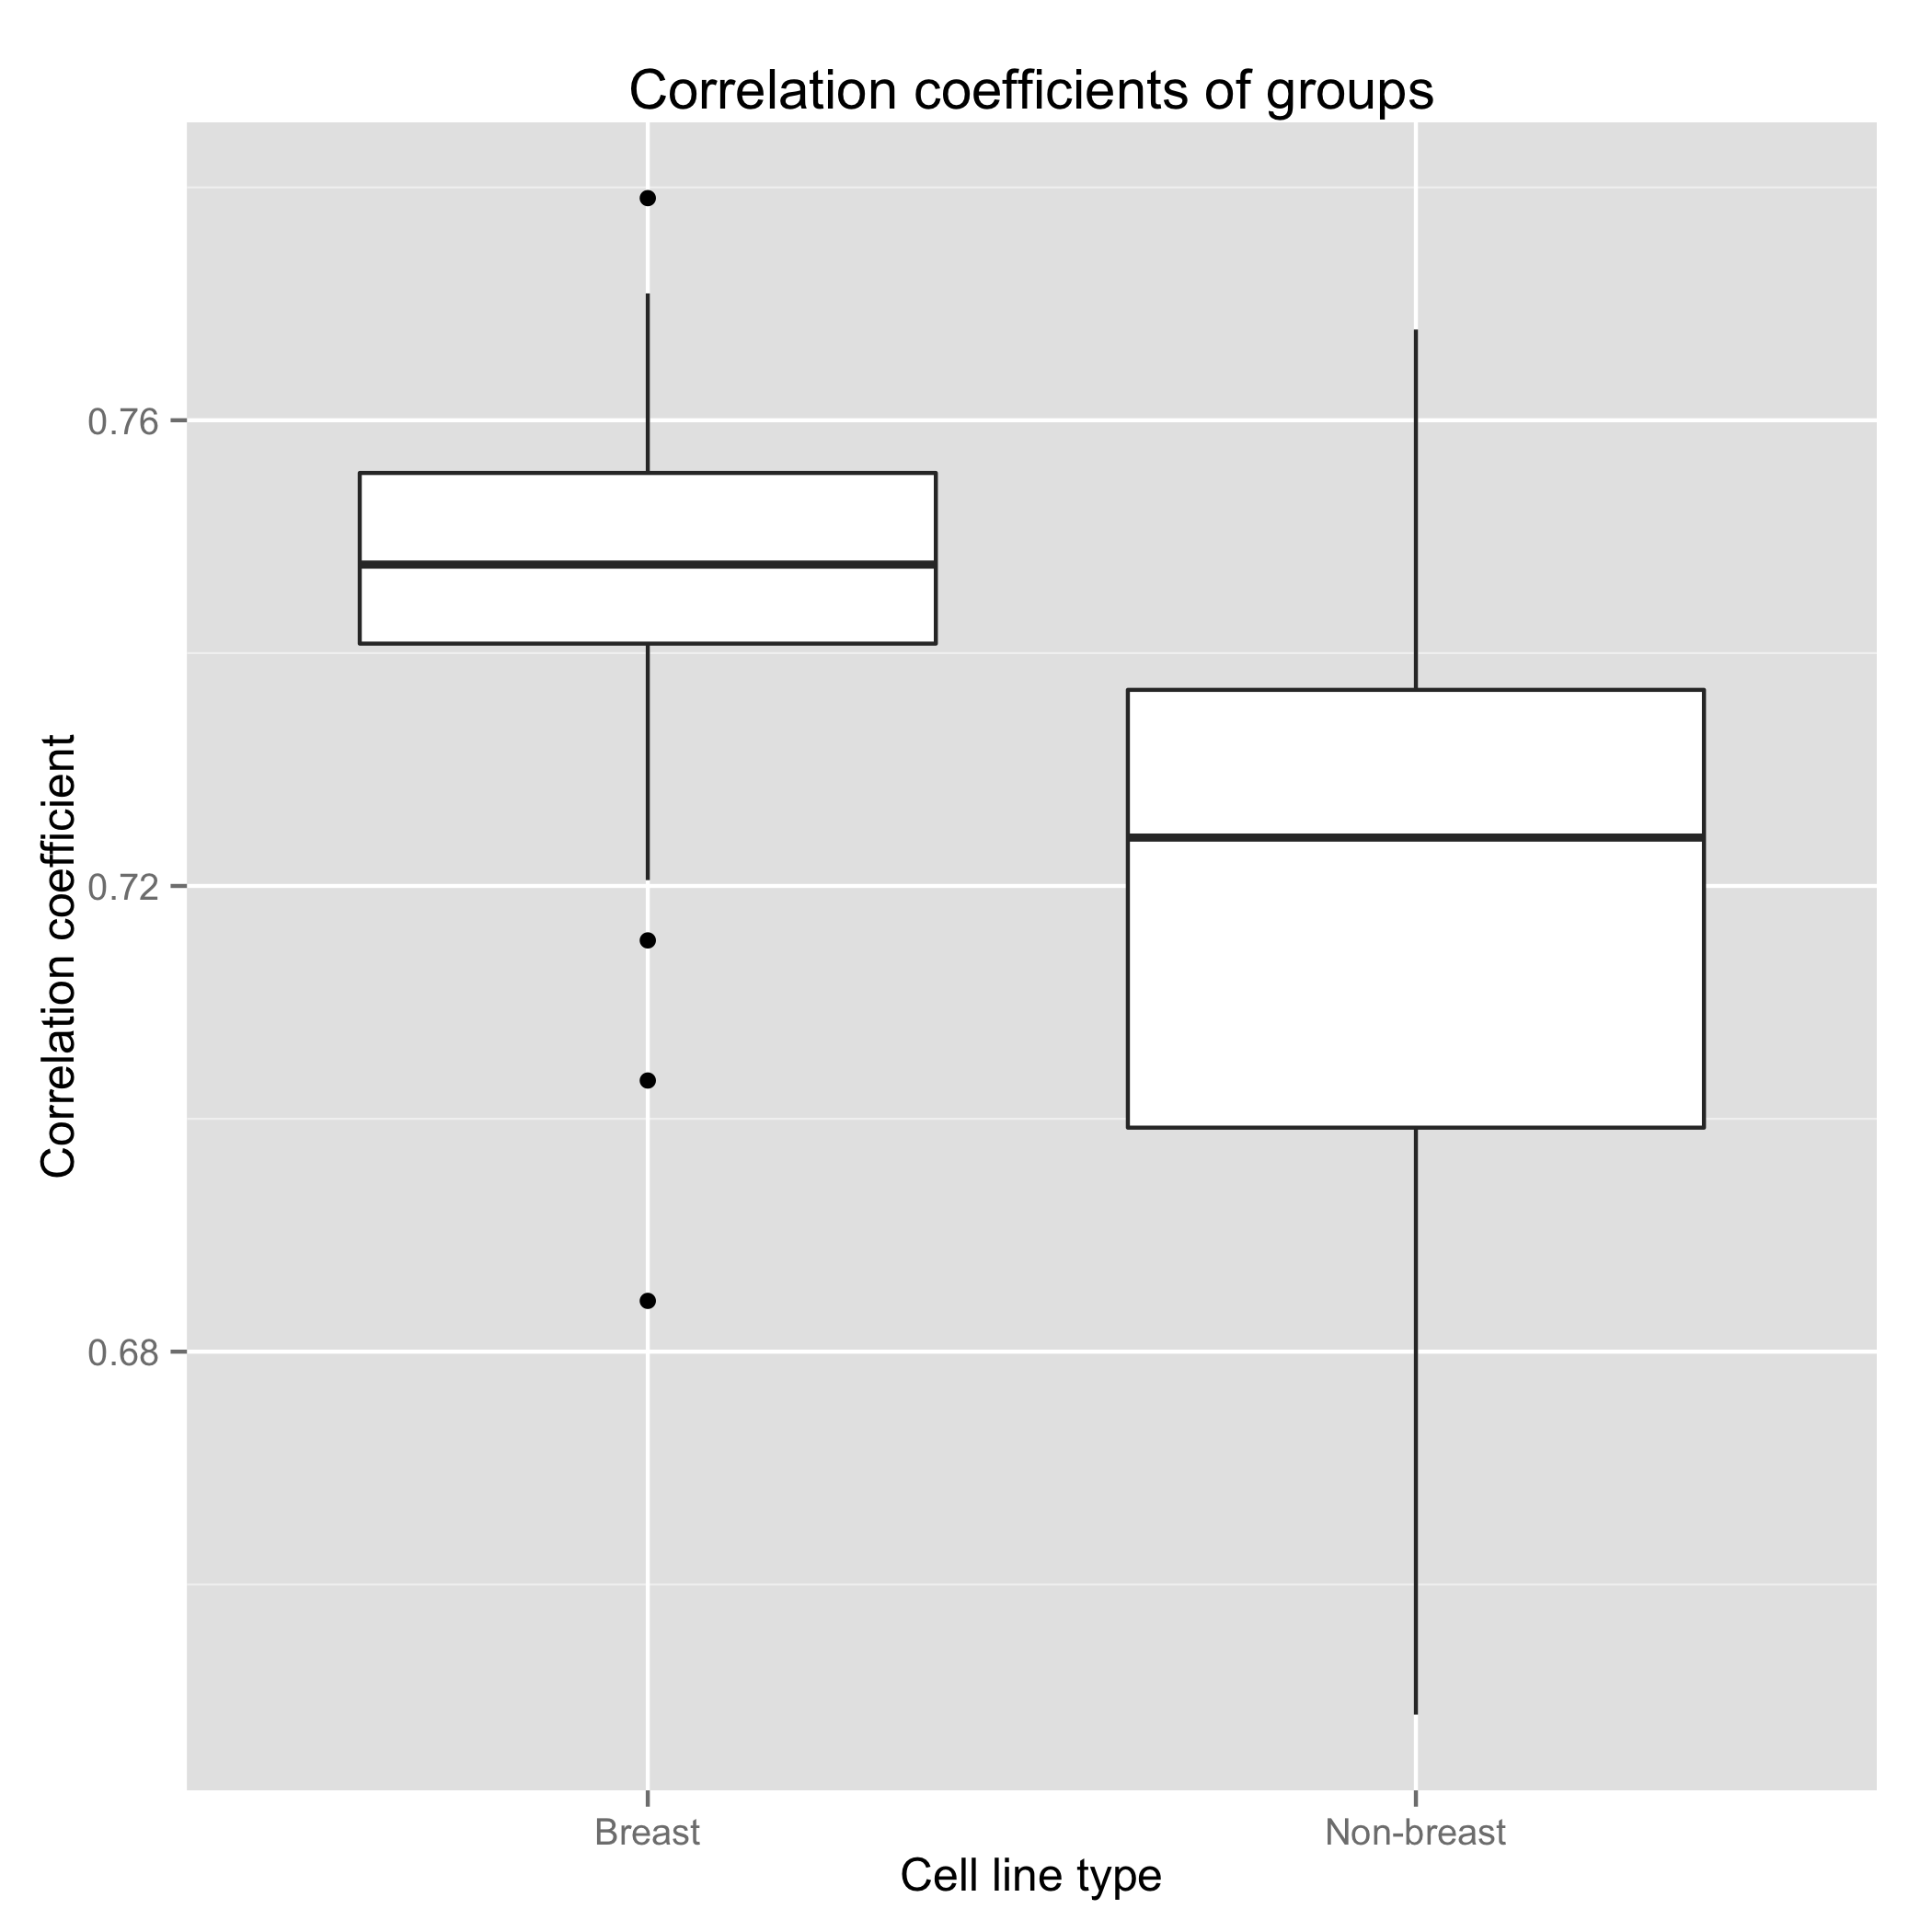
\includegraphics[width=7cm]{correlations.png}
\caption[Boxplot showing Spearman $\rho$ of cell lines from breast and
non-breast origin]{Boxplot showing the Spearman $\rho$ between
  $\textit{TGF}$-$\beta$ sensitive tumor model and cell lines from
  CCLE. Cell lines from CCLE have been divided into being of breast
  (left) and non-breast (right) origin. The mean correlation of the
  samples of breast origin is 0.75, while the mean correlation of
  samples of non-breast origin is 0.71. The difference is reported to
  be significant (p$<$0.001, wilcoxon ranked test)}
\label{rho}
\end{figure}
\subsection{CNV analysis using Pearson $\textit{r}$ shows low
  correlation between cell lines and tumor samples}
Copy number variations is a common hallmark of cancer, with agreement
that recurrent aberrations occur at loci containing genes that are
important for tumor development. In breast cancer, common aberrations
includes the amplification of regions containing $\textit{PIK3CA}$, $\textit{EGFR}$,
$\textit{FOXA1}$, $\textit{HER2}$ and deletions of regions containing
$\textit{MLL3}$, $\textit{PTEN}$,  $\textit{RB1}$ and
$\textit{MAP2K4}$ (TCGA, 2012).
Similar to Domcke et al, we adopted the Pearson $\textit{r}$ as a
measure of similarity to compare the CNV profiles of tumor and cell
lines. Strikingly, although those cell lines of breast origins are
sighnificantly more correlated (Figure \ref{cnv}), the mean
correlation is only 0.27, which is low.
\begin{figure}[t!]
\centering
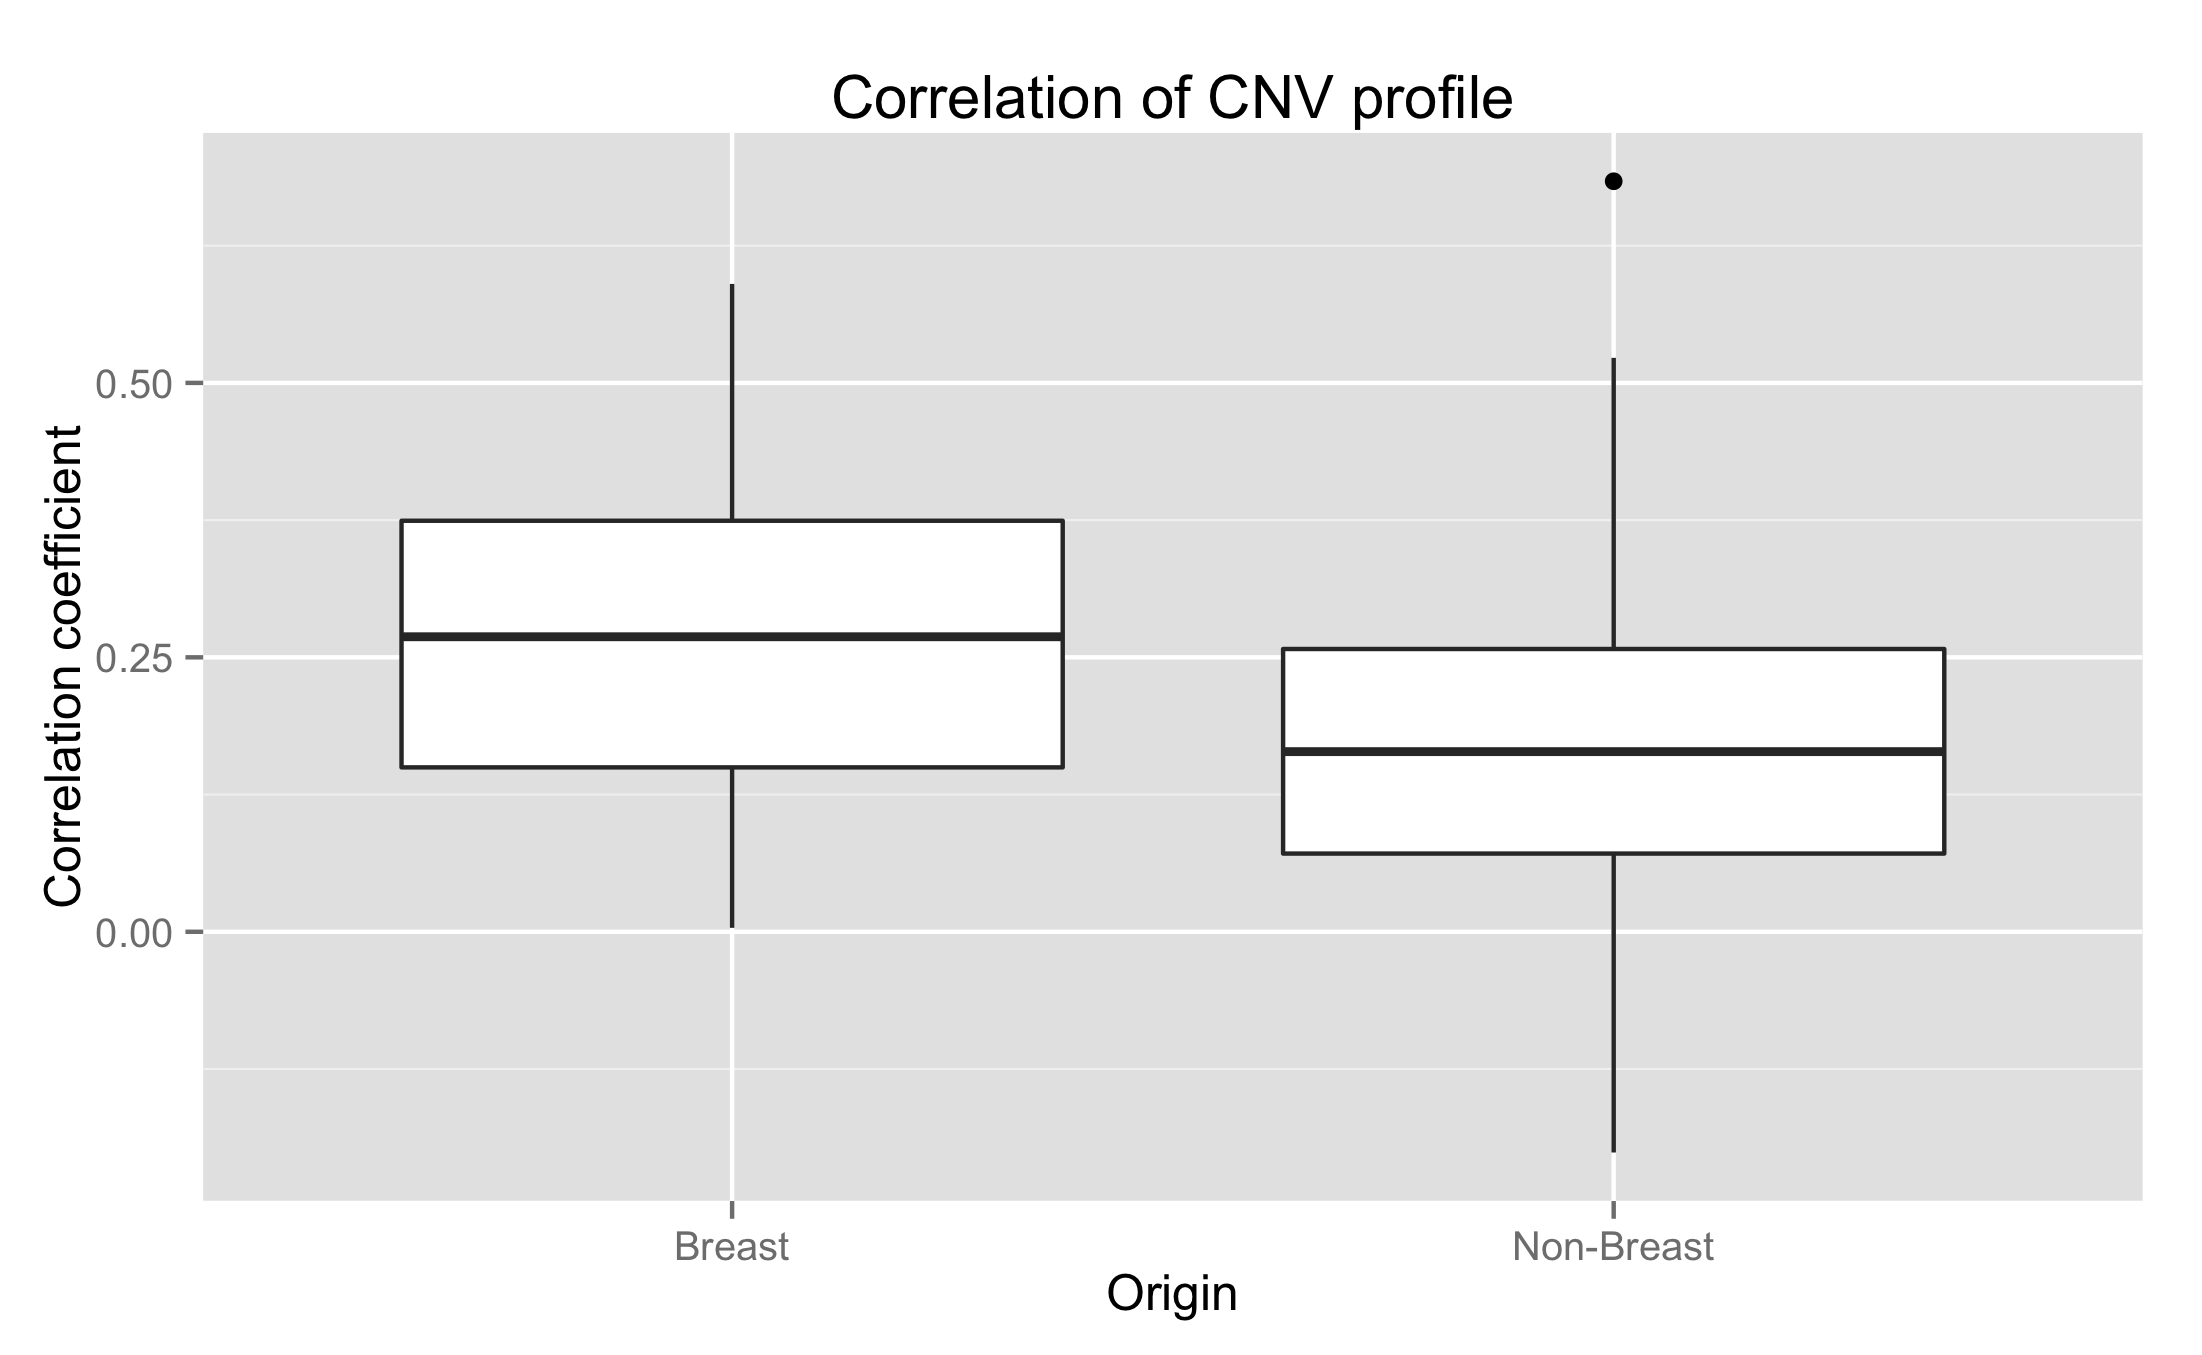
\includegraphics[width=7cm]{CNVcorrelations.png}
\caption[Boxplot showing Pearson $\textit{r}$ of cell lines from
breast and non-breast origin]{Boxplot showing the Pearson $\textit{r}$
between   $\textit{TGF}$-$\beta$ sensitive tumor model and cell lines from
  CCLE. Cell lines from CCLE have been divided into being of breast
  (left) and non-breast (right) origin. The difference is reported to
  be significant (p $<$0.001, wilcoxon ranked test), although the overall
correlation remains low.}
\label{cnv}
\end{figure}
Interestingly, when examining the CNV landscape of the tumors which
have been identified as being $\textit{TGF}$-$\beta$ sensitive - and
in particular, the 7 mentioned CNVs that are consistently aberrated,
we note that are huge variability (Figure \ref{cnvlandscape}), with
reported standard deviations between 0.23 and 0.35. Strikingly, the
gene $\textit{MLL3}$, which is reported to be deleted in breast
cancer, was noted to have marginal amplifications instead (mean=
0.0266,median=0.0337,$\sigma$=0.273).
\begin{figure}[t]
\centering
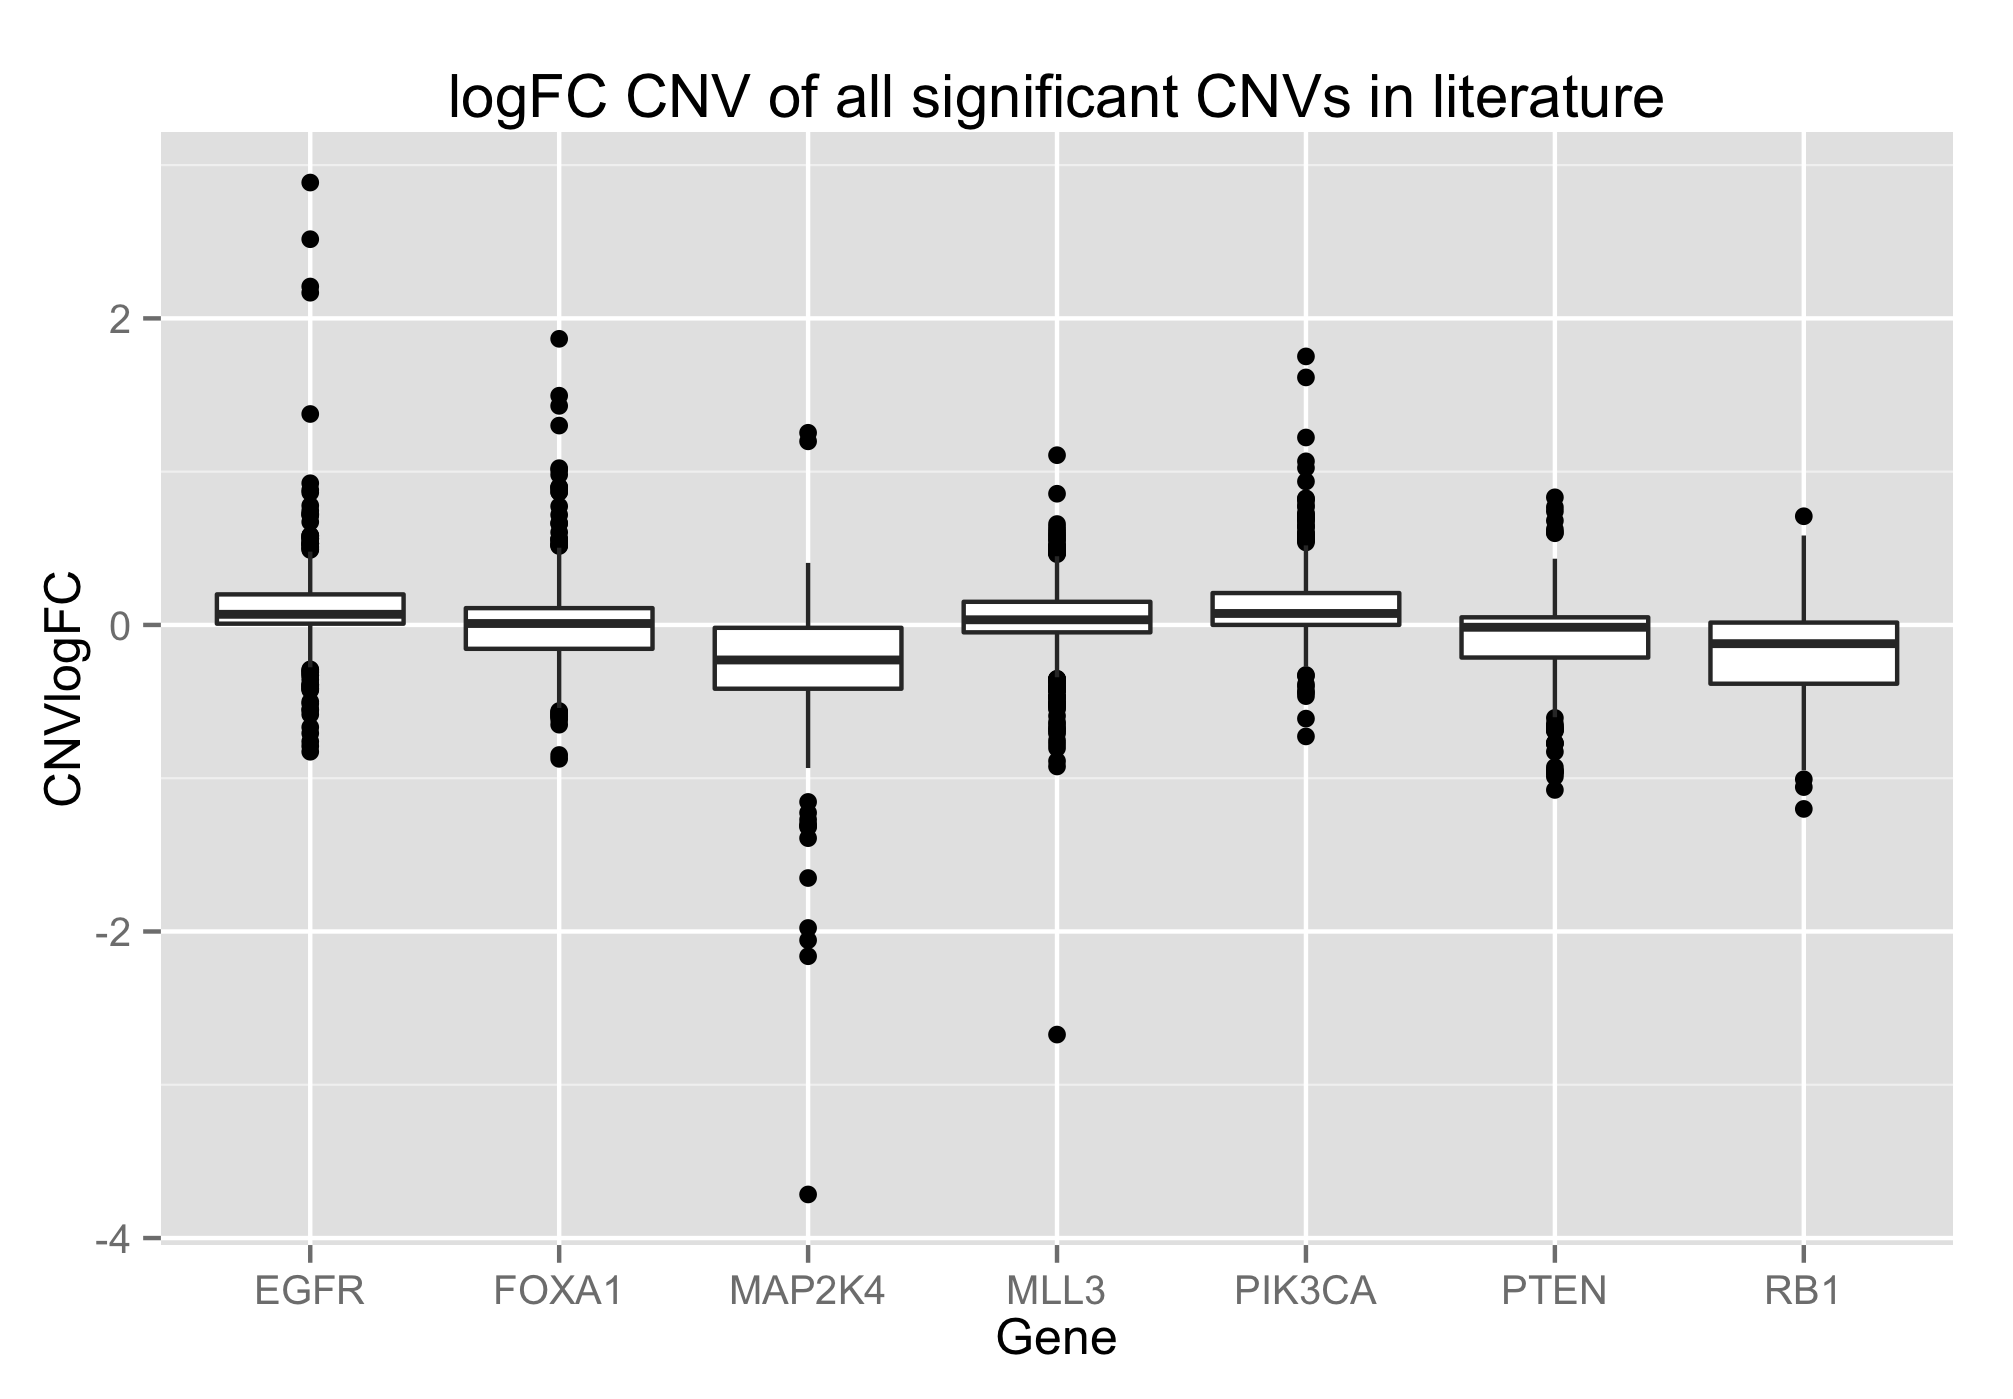
\includegraphics[width=7cm]{CNVreported.png}
\caption[Boxplot showing CNVs of 7 genes in TCGA identified as being
aberrated]{Boxplot showing the CNVs of 7 genes confirmed as being
  aberrated - either by amplification
  ($\textit{PIK3CA}$,$\textit{EGFR}$,$\textit{FOXA1}$,$\textit{HER2}$)
  or deletion
  ($\textit{PTEN}$,$\textit{RB1}$,$\textit{MLL3}$,$\textit{AMP2K4}$). Overall
  the copy number variations appear to be flat, but with large
  variations observed among all 568 samples.}
\label{cnvlandscape}
\end{figure}
When we compare the CNV landscape of the 7 genes between TCGA and CCLE
data, we find that they are largely identical (Figure \ref{cnvcompare})
\begin{figure}[h]
\centering
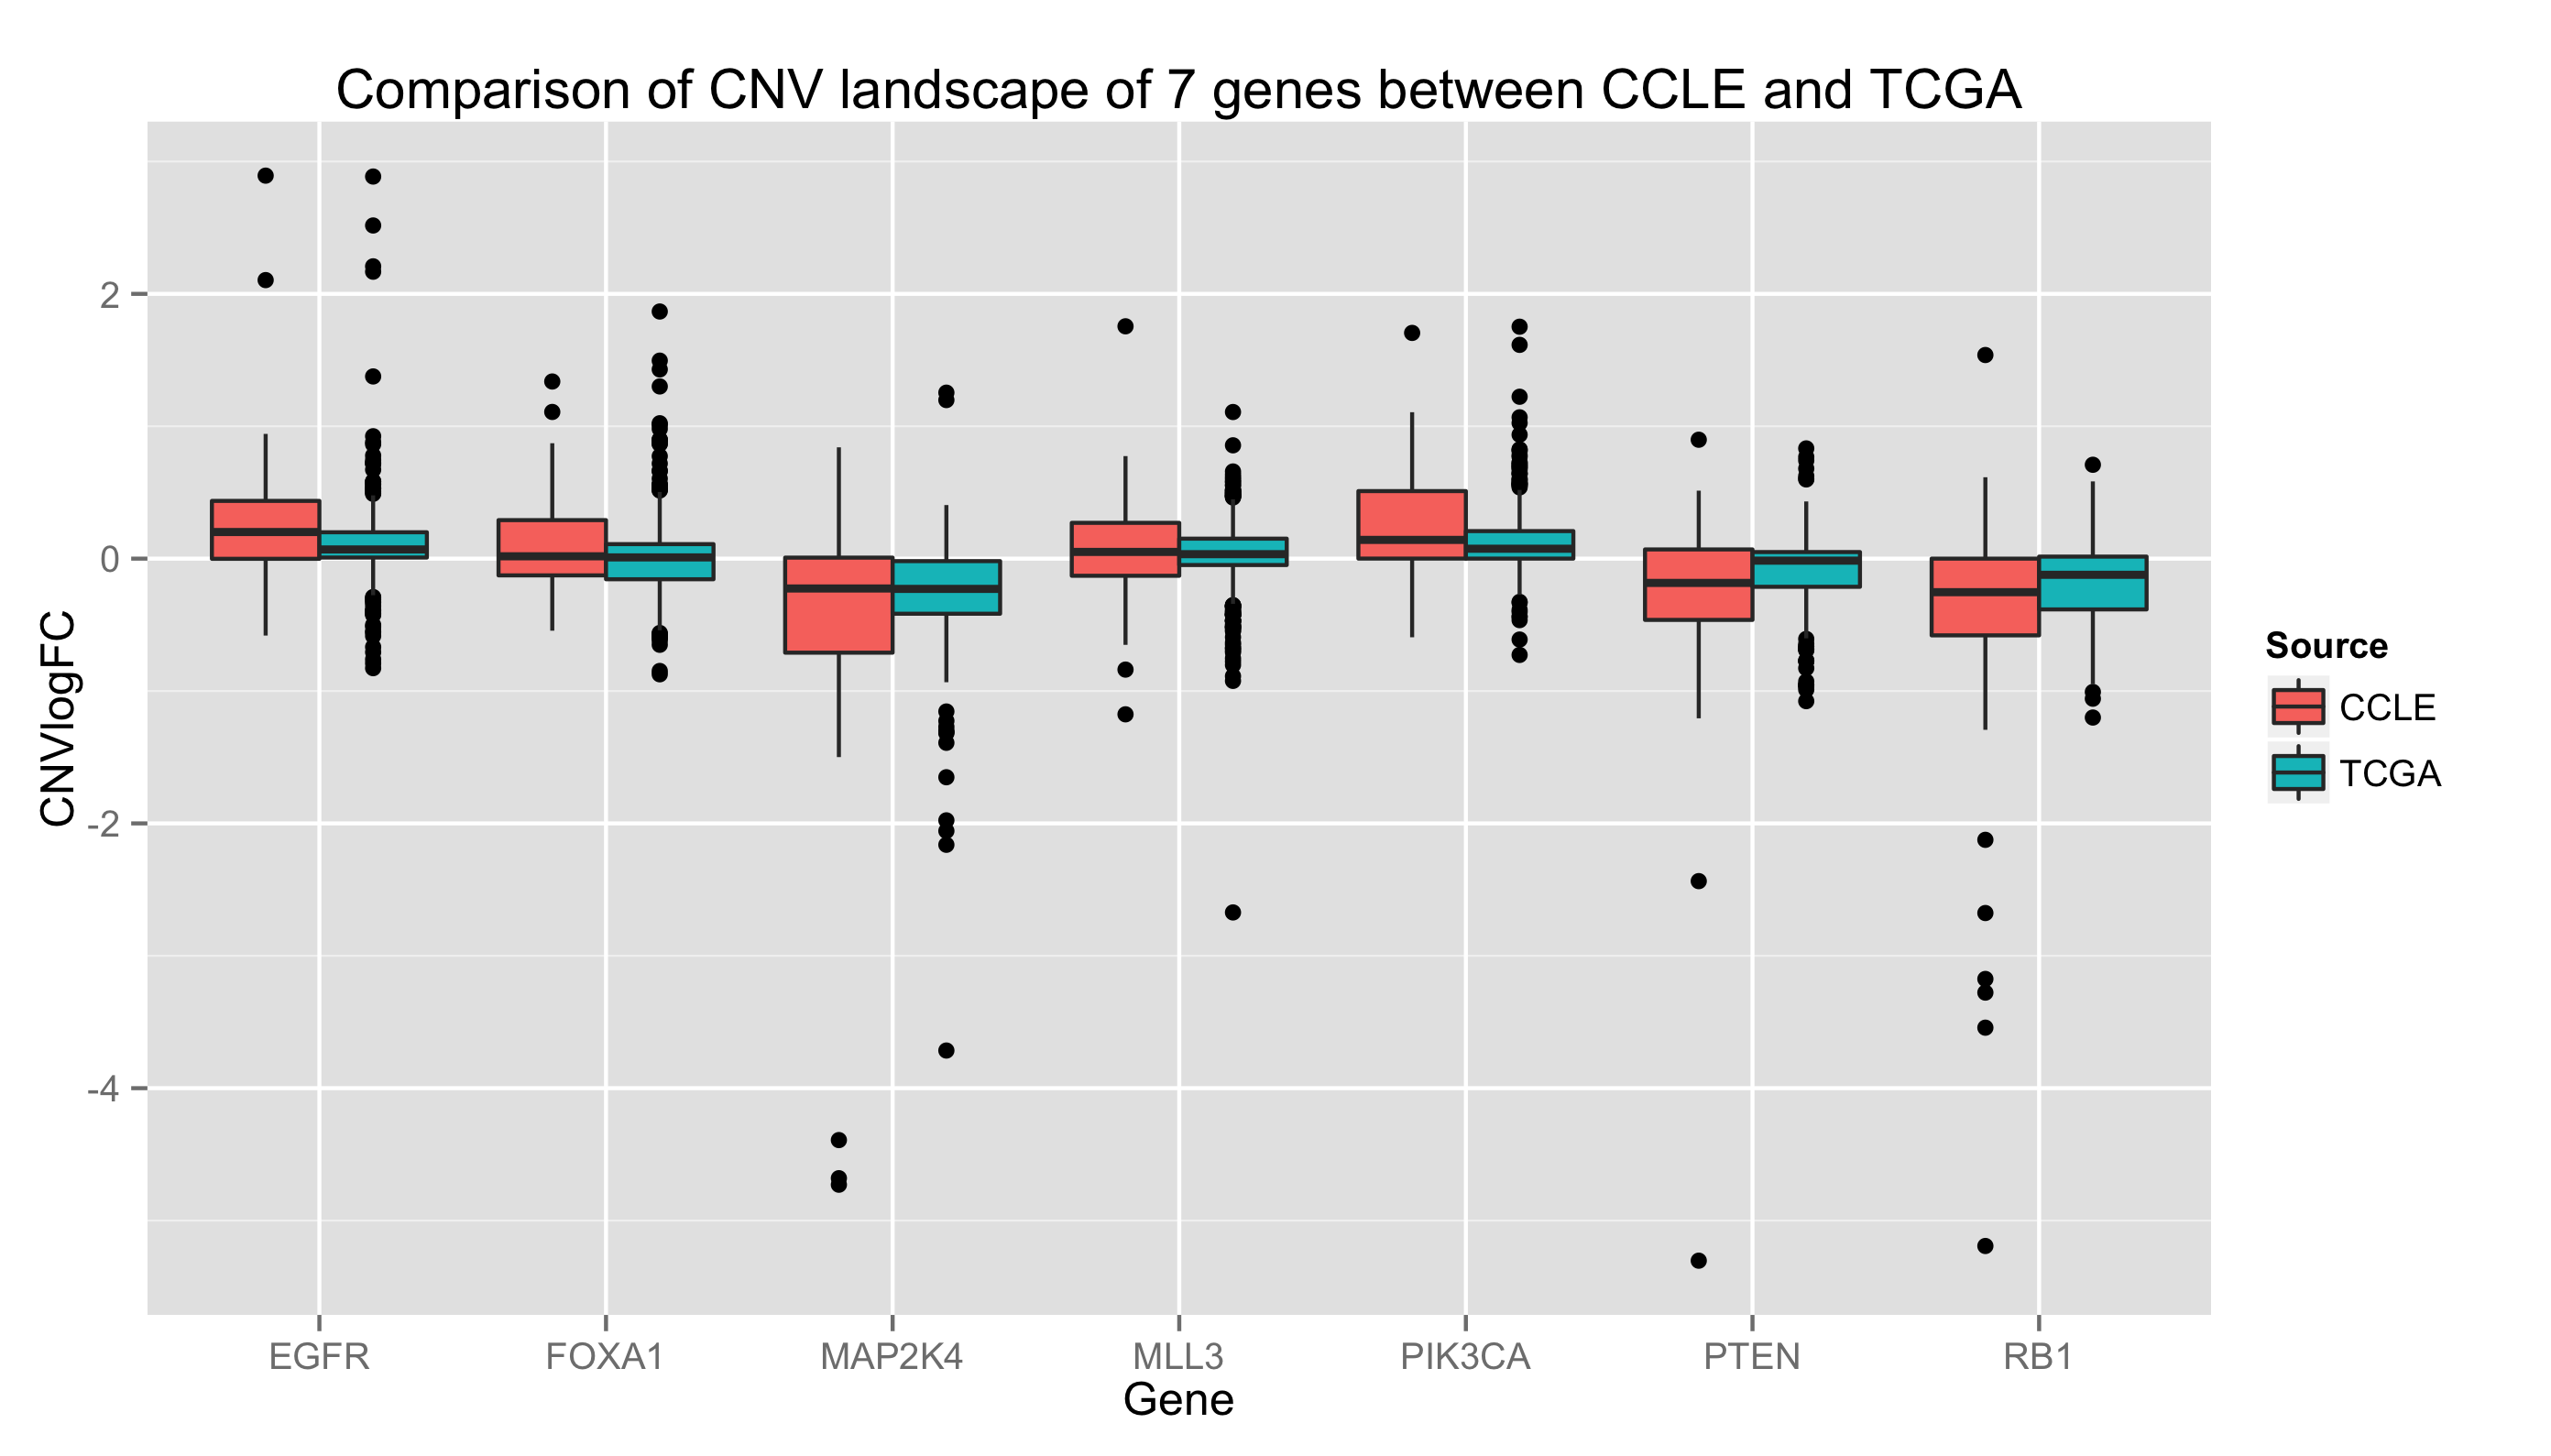
\includegraphics[width=9cm]{CNVcomparison.png}
\caption[Boxplot comparing CNV landscape of CCLE and TCGA data at 7
gene loci]{Boxplot showing the CNV landscape of CCLE and TCGA samples
  at 7 loci identified as being consistently aberrated- either by amplification
  ($\textit{PIK3CA}$,$\textit{EGFR}$,$\textit{FOXA1}$,$\textit{HER2}$)
  or deletion
  ($\textit{PTEN}$,$\textit{RB1}$,$\textit{MLL3}$,$\textit{AMP2K4}$). The
distribution of CNVs appear to be identical, with relatively flat landscapes}
\label{cnvcompare}
\end{figure}
Given these CNVs have been reported in breast cancer, we expect that
the CNV profiles at these 7 loci be largely consistent between both
TCGA and CCLE data, as shown in Figure \ref{cnvcompare}. Thus, the low
correlation appears to be due to changes in the global CNV
distribution which might be unique to the $\textit{TGF}$-$\beta$
sensitive system.

\subsection{The mutational landscape of tumor samples is highly
  heterogeneous}
Consistent with earlier reports, the mutation landscape of breast
cancer is highly heterogeneous, with few mutations found in $>$10\% of
the samples (Figure \ref{distribution}), while table \ref{mutations}
below shows the most common occurring mutations that were observed in
the TCGA dataset of 936 breast cancer samples.
\begin{figure}
\centering
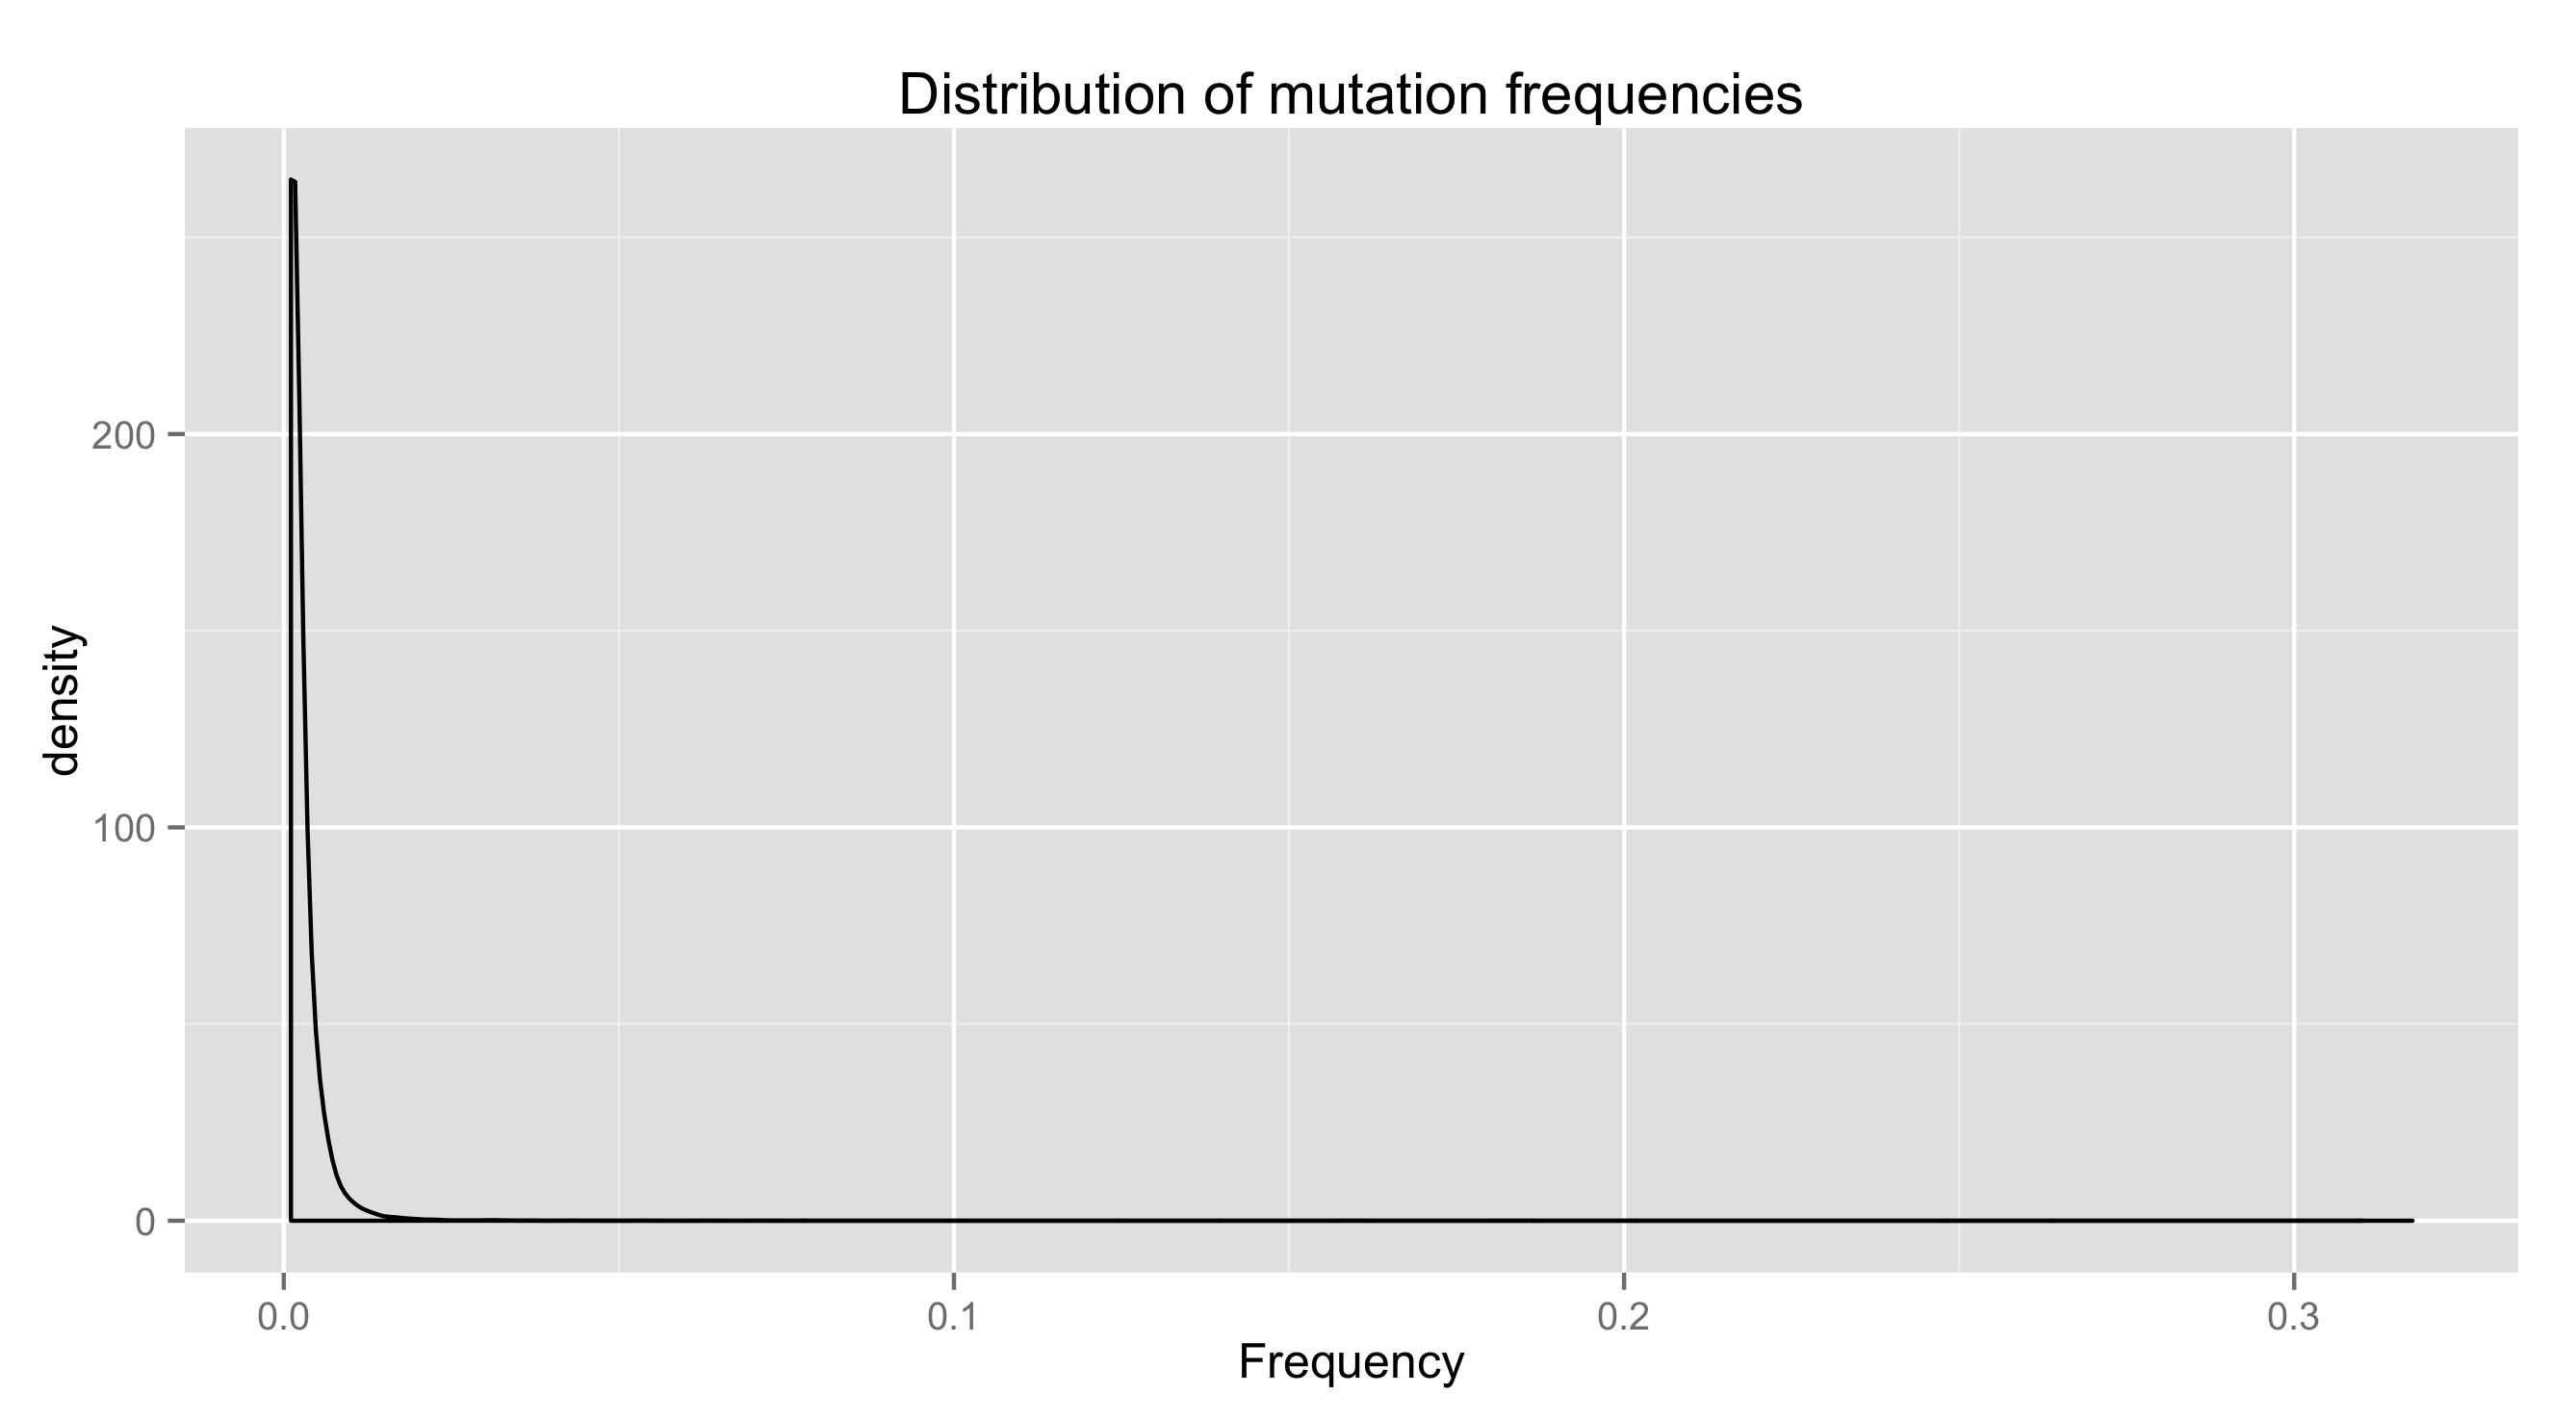
\includegraphics[width=9cm]{distribution.png}
\caption[Density plot of somatic mutations in breast cancer]{Density
  showing the frequency of somatic mutations occurring in breast
  cancer. The frequencies are derived from the TCGA dataset of 936
  samples. The heterogeneity of the mutational landscape is shown by
  the left-skew of the distribution, where each mutation occurs at
  very small frequencies}
\label{distribution}
\end{figure}

\begin{table}
\caption{Table showing the more common mutations in breast cancer,
  occuring in $>$10 \% of all breast cancer samples}
\label{mutations}
\begin{tabular}{c c}
\hline
Mutation&Observed Frequency \\
\hline
$\textit{TP53}$ Missense Mutation & 0.1828877 \\
$\textit{TTN}$ Missense Mutation & 0.1593583 \\
$\textit{PIK3CA}$ Missense Mutation & 0.3176471 \\
\hline
\end{tabular}
\end{table}
That $\textit{TP53}$ is commonly mutated is hardly surprising, as it
is estimated to be found in approximately 50\% of human
cancers. However, studies have shown that in the case of breast
cancer, the frequency of $\textit{TP53}$ is about 20\%, although this
is highly dependent on the type and staging of the breast cancer
(\cite{Pharoah1999}. This value of 20\% agrees well with our
observation that $\textit{TP53}$ mutations occurring in about 18\% of
breast cancer cases. Similarly, our observation of $\textit{PIK3CA}$
having the highest mutation is also consistent with literature, and
has been estimated to be mutated in 20\% - 40\% of breast cancer cases
\cite{Cizkova2012}. Likewise, our observation of $\textit{TTN}$
being commonly mutated is also confirmed by earlier studies to be a
potential oncogene \cite{Greenman2009}.

\subsection{Use of conditional probabilities in comparing somatic
  mutations lends an intuitive interpretation}
The use of a conditional probability,
P($\textit{X}$$\mid$$\textit{Y}$) lends itself to intuitive
interpretation. The probability, $\textit{p}$ can be understood to be
the probability of a given sample being  $\textit{TGF}$-$\beta$
sensitive model given the spectrum of mutation that it possess. The
frequency of the mutations occurring - either among breast cancer, or
among $\textit{TGF}$-$\beta$ sensitive sample - is informed by the
available data. A $\textit{p}$ of 1 - or a sure event - means that
given the amount of information we have before hand, we can be sure
that the cell line is of a $\textit{TGF}$-$\beta$ sensitive origin.

From the available data, we derive the priors and a few of the more
important frequencies which we use for the computation of the
posterior conditional probability. These values are shown in Table \ref{probs}.

\begin{table}[b]
\caption{Table showing some crucial values involved in calculating the
posterior conditional probability P($\textit{X}$$\mid$$\textit{Y}$)}
\label{probs}
\begin{tabular}{c c c}
  \hline
  Symbol & Value & Interpretation\\
  \hline
  P($\textit{X}$) & 0.6068 & Probability of sample being classified
  as $\textit{TGF}$-$\beta$ sensitive\\
  \hline
\end{tabular}
\end{table}

\subsection{Bayesian conditional probabilities suggests that
  the mutational landscape of cell lines have undergone significant
  changes}
The conditional probability, P($\textit{X}$$\mid$$\textit{Y}$)
(Eq. 4), denotes the probability of a cell line being
$\textit{TGF}$-$\beta$ sensitive given that it contains a specific
set of mutation. Table \ref{pxy} shows the probability for the top 5
breast cancer cell lines, alongside their correlation to the CNV and
gene expression profile of TCGA sample.
\begin{table}
\caption[Table showing scores of the top 5 breast cell lines and
associated scores ]{Table
  showing the conditional probabilities
  P($\textit{X}$$\mid$$\textit{Y}$) of the top 5 BC cell lines, as well as
  correlations of CNV and gene expression that derive their total scores}
\label{pxy}
\begin{tabular}{l  c  c  c c}
\hline
Cell line & Correlation(CNV) & Correlation(GE) &
P($\textit{X}$$\mid$$\textit{Y}$) & Score \\
\hline
HCC2157 & 0.4470866 & 0.7326566 & 6.492890e-02 & 3.244672\\
HCC1569 & 0.4692470 & 0.7374384 & 1.265671e-04 & 3.206812\\
HCC70   & 0.3631997 & 0.7548653 & 6.492890e-02 & 3.182994\\
SKBR3   & 0.3477014 & 0.7583189 & 6.492890e-02 & 3.170949\\
DU4475  & 0.4834161 & 0.6843618 & 6.492890e-02 & 3.167787\\
\hline
\end{tabular}
\end{table}
Interesting, despite the relatively high correlation in terms of gene
expression, the mutation scores (P($\textit{X}$$\mid$$\textit{Y}$)) are
generally small. There are 2 possible reasons for such an
observation. On one hand, it might be due to the fact that only 33
genes were used to derive the mutation scores.

\subsection{Scoring scheme suggests HCC2157 as the best cell line model}
Table \ref{pxy} shows the scores of the top 5 breast cancer cell line
models that would be $\textit{TGF}$-$\beta$ sensitive, and suggests
the cell line HCC2157 as the best cell line model. The cell line is
shown to have a high correlation in terms of gene expression and copy
number aberrations, while also having the highest probability of being
$\textit{TGF}$-$\beta$ sensitive given its mutational profile.
Interestingly, our scoring scheme also suggests a few other cell lines
that appear to be closely related to the system of our interest,
namely, $\textit{TGF}$-$\beta$ sensitive breast cancer. Table \ref{top10} shows the top 10 cell line models from our scoring scheme
\begin{table}
\caption[Table showing scores of top 10 cell lines ]{Table showing the
top 10 cell lines that best resembles $\textit{TGF}$-$\beta$ sensitive
breast cancer}
\label{top10}
\begin{tabular}{l  c c  c  c c}
\hline
Cell line & Origin & Corr(CNV) & Corr(GE) &
P($\textit{X}$$\mid$$\textit{Y}$) & Score \\
\hline
HCC2157 & Breast & 0.4470866 & 0.7326566 & 6.492890e-02 & 3.244\\
HCC1569 & Breast & 0.4692470 & 0.7374384 & 1.265671e-04 & 3.206\\
NCIH1666& Lung & 0.4482049 & 0.7443055 & 9.492530e-06 & 3.192\\
HCC70   & Breast & 0.3631997 & 0.7548653 & 6.492890e-02 & 3.182\\
WM88    & Skin & 0.4581817 & 0.7234239 & 9.492530e-06 & 3.181\\
COLO704 & Ovary & 0.5040814 & 0.6743619 & 5.695518e-05 & 3.178\\
SKBR3   & Breast & 0.3477014 & 0.7583189 & 6.492890e-02 & 3.170\\
DU4475  & Breast & 0.4834161 & 0.6843618 & 6.492890e-02 & 3.167\\
SNU245  & Biliary tract & 0.3431889 & 0.7201723 & 6.492890e-02 & 3.128\\
A2058   & Skin & 0.3796327 & 0.7439474 & 9.492530e-06 & 3.123\\
\hline
\end{tabular}
\end{table}

\subsection{Future works}
Further improvements to the scoring scheme can be conceived to also
include epigenetic information as they become available for cell
lines, as CCLE currently does not contain such information.
Likewise, as another possible improvement to the scoring scheme
involves the refinement of the mutation scores. On this front, 2
possible improvements can be suggested. Firstly, the global mutation
landscape of the cell lines should be considered in our scoring
scheme, as this will be more informative in light of the genomic
heterogeneity of cancers. Secondly, the somatic mutation landscape of
cell lines tend to be different from those from tumor samples because
they are grown in artificial environments, and a refined scheme might
be cognizant of these differences.

\section{Conclusion}
In this present study, we have proposed modifications to the initial scoring
scheme proposed by Domcke et al in order to use genomic data to guide
the selection of cell lines in cancer research. Significantly, we
introduced a weighted scoring scheme for somatic mutations, as well as
taking into account the gene expression profile of both tumor and cell
lines. We then applied our method to identifying cell lines that are
most appropriate for the study of $\textit{TGF}$-$\beta$ sensitive
breast cancer.
\newpage
\addcontentsline{toc}{section}{Bibliography}
\bibliography{references}

\end{document}
